% automatically generated document using lt2circuiTikz
\documentclass[tikz,margin={2pt 2pt 2pt 2pt}]{standalone}
\usepackage[compatibility,siunitx,  americanvoltages, americancurrents, europeanresistors, europeaninductors, americanports,%
  straightlabels, fetbodydiode]{circuitikz}
\usepackage{tikz,amsmath, amssymb,bm,color,pgfkeys,siunitx,ifthen}
\usepackage{pgfplots}
\pgfplotsset{compat=1.14}
\usetikzlibrary{shapes,arrows}
\usepackage{agaramondc}					% Adobe Garamond, custom shape
\renewcommand{\shapedefault}{rtl} % rtl: roman tabular lining


\usetikzlibrary{backgrounds,calc,positioning}
%\draw (0,0) node[<CompName>,<Options,optional>] (<AnchorName,optional>) {<TextAtAnchor,optional>}; % curly brackets are mandatory, even if empty!
%\draw (<x1>,<y1>) to[<CompName>,<Options,optional>] (<x2>,<y2>);
\usetikzlibrary{circuits.ee.IEC}


% sym32a style

\ctikzset{tripoles/mos style/arrows}
\ctikzset{
	%/tikz/circuitikz/bipoles/length=1.2cm,%1.4cm
	%/tikz/circuitikz/tripoles/pigfetd/height=1.363,%1.1
	%/tikz/circuitikz/tripoles/pigfetd/width=0.8674, %0.7
	%/tikz/circuitikz/tripoles/nigfetd/height=1.363,%1.1
	%/tikz/circuitikz/tripoles/nigfetd/width=0.8674, %0.7
	%/tikz/circuitikz/tripoles/nigfete/height=1.363,%1.1
	%/tikz/circuitikz/tripoles/nigfete/width=0.8674, %0.7
	%/tikz/circuitikz/tripoles/pigfete/height=1.363,%1.1
	%/tikz/circuitikz/tripoles/pigfete/width=0.8674, %0.7
	%%	%
	%/tikz/circuitikz/tripoles/npn/height=1.363,%1.1
	%/tikz/circuitikz/tripoles/npn/width=0.7435, %0.6
	%/tikz/circuitikz/tripoles/pnp/height=1.363,%1.1
	%/tikz/circuitikz/tripoles/pnp/width==0.7435, %0.6
	/tikz/circuitikz/bipoles/diode/height=0.375,%
	/tikz/circuitikz/bipoles/diode/width=0.375,%
	/tikz/circuitikz/tripoles/op amp/height=0.952,%
	/tikz/circuitikz/tripoles/op amp/width=1.2,%
	/tikz/circuitikz/tripoles/op amp/font=\footnotesize,
}

\begin{document}%
	%\centering%
	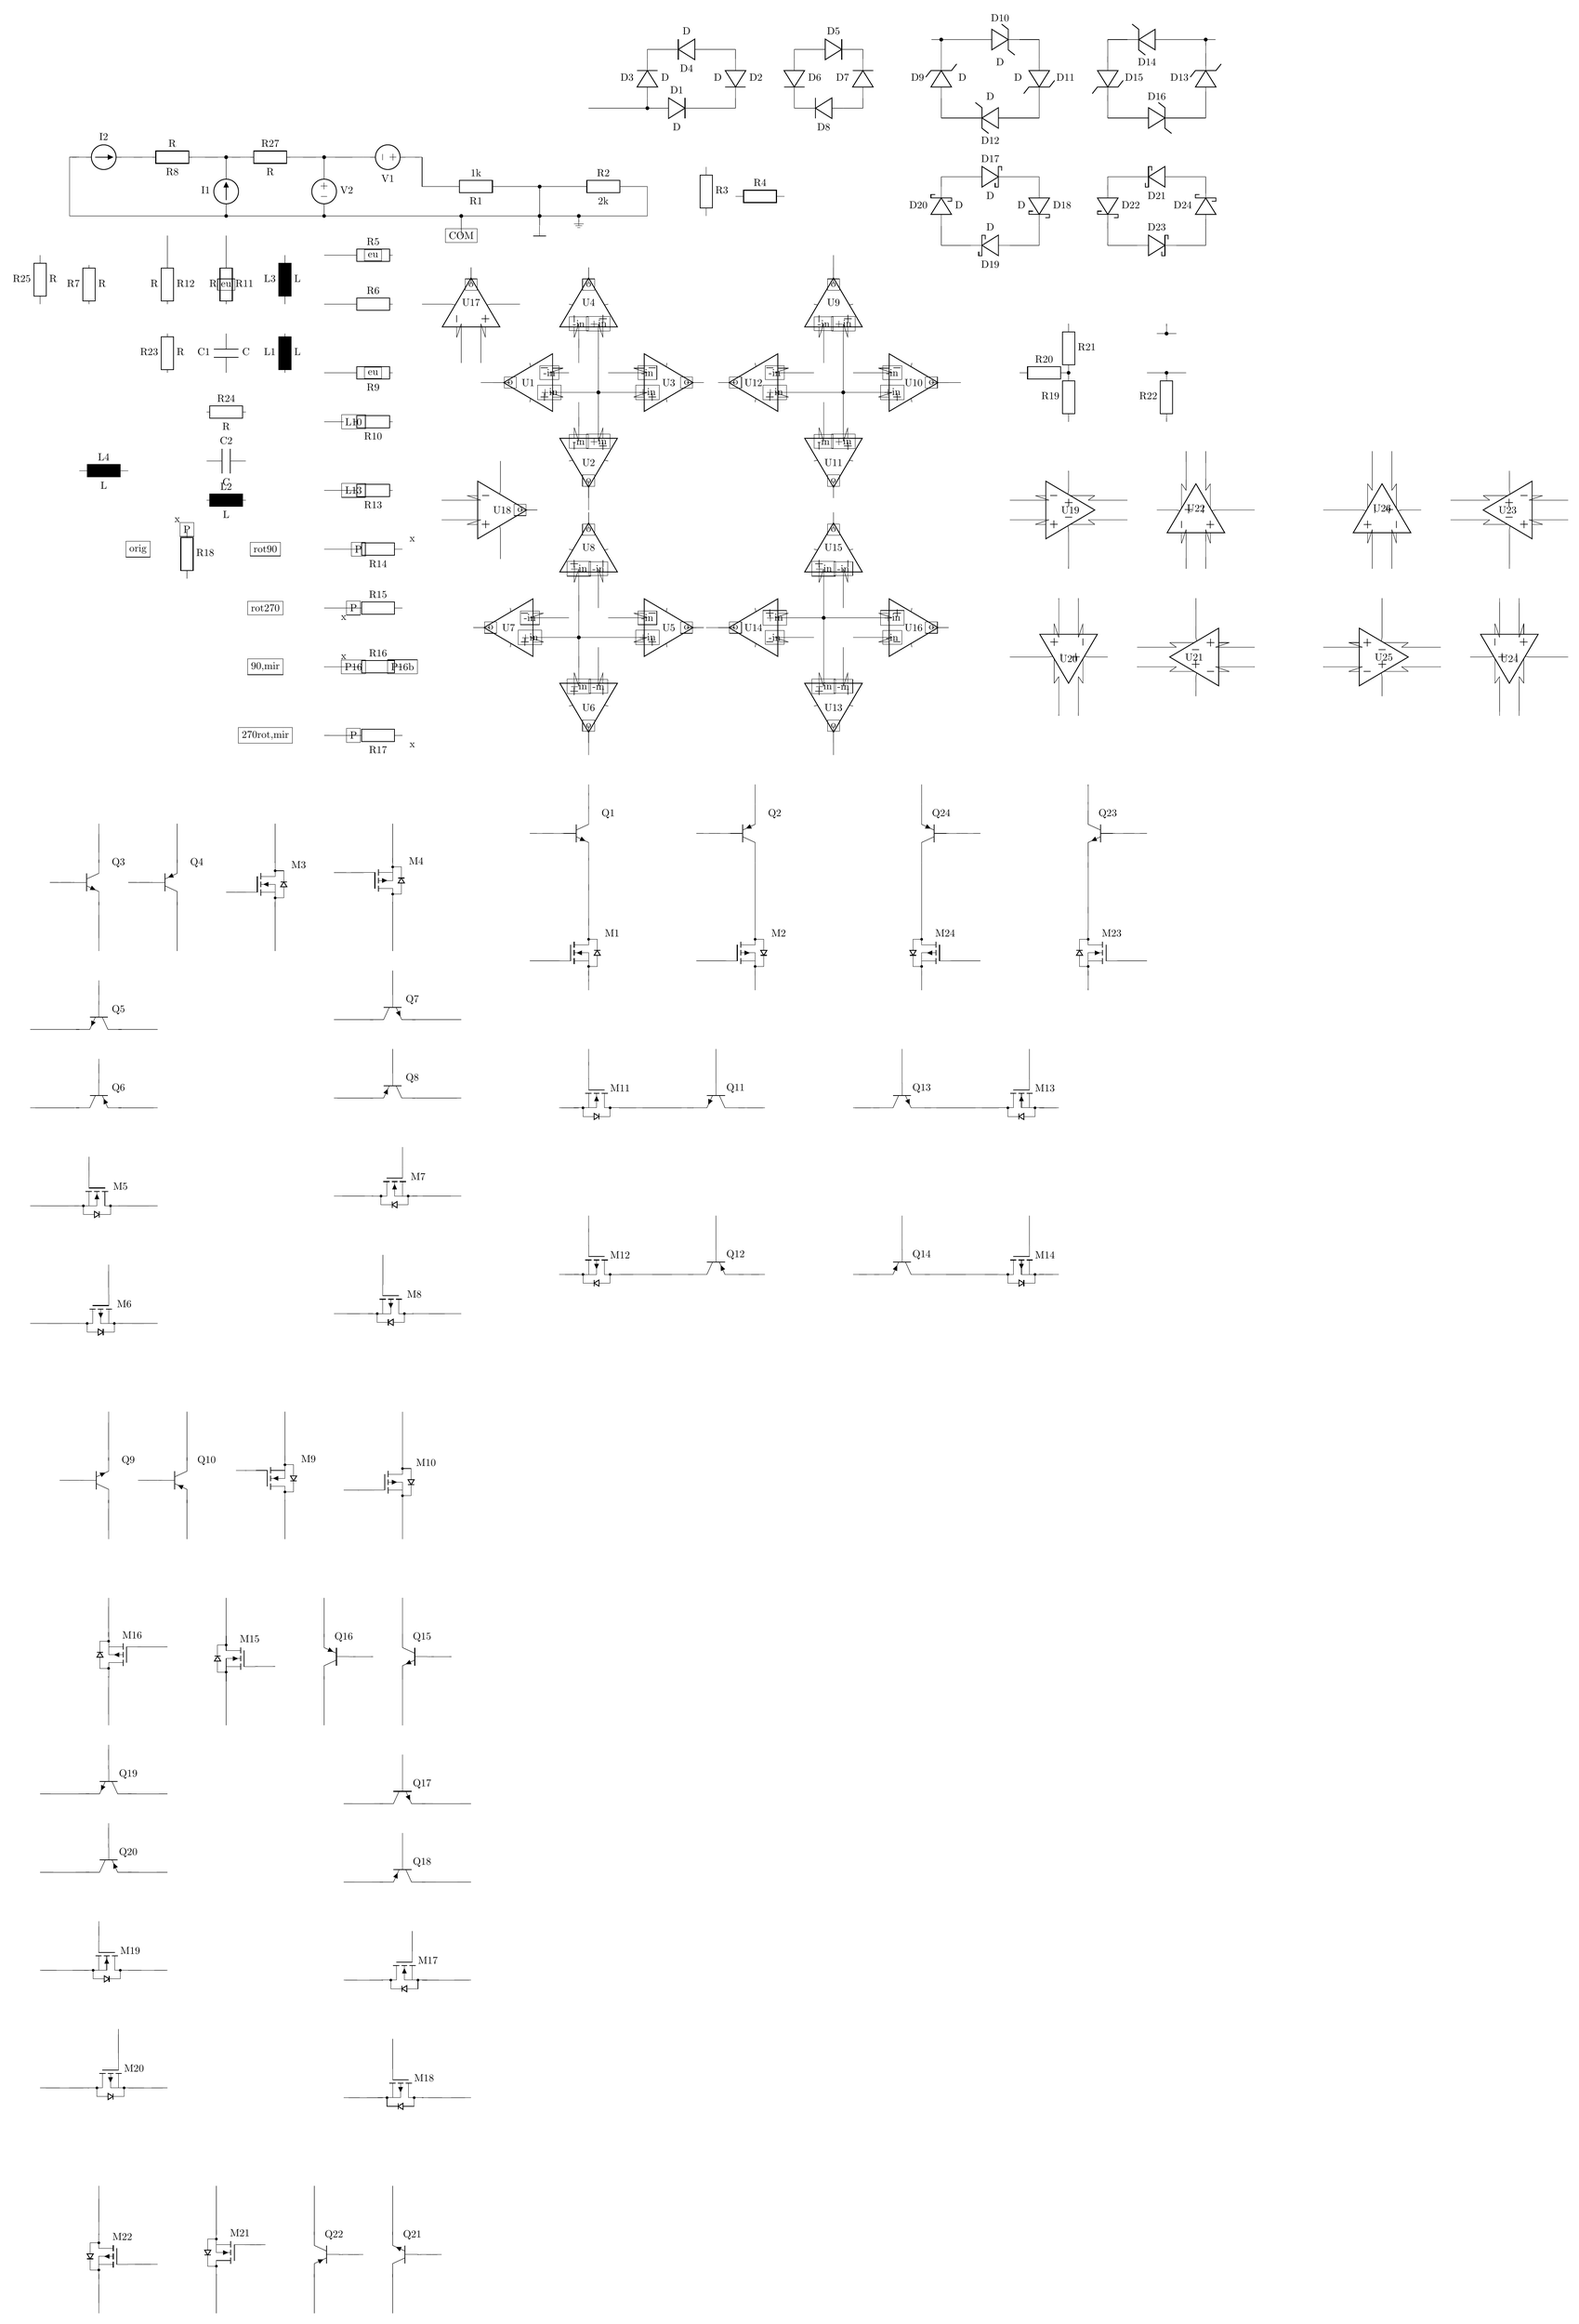
\begin{tikzpicture}[circuit ee IEC, scale=0.6666666667]%
	%\tikzstyle{every node}=[font=\small];%
	%\node [draw] at (0.0,0.0) {\pgfkeysvalueof{/tikz/circuitikz/tripoles/op amp/font}};
\draw (27.5,4.0)to[*short,*-] (27.0,4.0);% wire w3
\draw (29.5,4.0)to[*short,-*] (27.5,4.0);% wire w4
\draw (37.0,4.0)to[*short,-] (36.0,4.0);% wire w6_w19 start
\draw (36.0,4.0)to[*short,-] (36.0,3.0);% wire w6_w19 end
\draw (37.0,4.0) --  (36.0,4.0) -- (36.0,3.0); % wire w6_w19 polyline 
\draw (41.0,4.0)to[*short,*-] (39.0,4.0);% wire w7
\draw (41.5,4.0)to[*short,-*] (41.0,4.0);% wire w8
\draw (13.5,3.5)to[*short,-] (12.5,3.5);% wire w9_w13 start
\draw (12.5,3.5)to[*short,-] (12.5,3.0);% wire w9_w13 end
\draw (13.5,3.5) --  (12.5,3.5) -- (12.5,3.0); % wire w9_w13 polyline 
\draw (21.0,3.5)to[*short,-] (20.0,3.5);% wire w11_w15 start
\draw (20.0,3.5)to[*short,-] (20.0,3.0);% wire w11_w15 end
\draw (21.0,3.5) --  (20.0,3.5) -- (20.0,3.0); % wire w11_w15 polyline 
\draw (17.0,3.0)to[*short,-] (17.0,3.5);% wire w10_w14 start
\draw (17.0,3.5)to[*short,-] (15.5,3.5);% wire w10_w14 end
\draw (17.0,3.0) --  (17.0,3.5) -- (15.5,3.5); % wire w10_w14 polyline 
\draw (23.5,3.0)to[*short,-] (23.5,3.5);% wire w12_w16 start
\draw (23.5,3.5)to[*short,-] (23.0,3.5);% wire w12_w16 end
\draw (23.5,3.0) --  (23.5,3.5) -- (23.0,3.5); % wire w12_w16 polyline 
\draw (27.5,3.0)to[*short,-*] (27.5,4.0);% wire w17
\draw (32.5,3.0)to[*short,-] (32.5,4.0);% wire w5_w18 start
\draw (32.5,4.0)to[*short,-] (31.5,4.0);% wire w5_w18 end
\draw (32.5,3.0) --  (32.5,4.0) -- (31.5,4.0); % wire w5_w18 polyline 
\draw (41.0,3.0)to[*short,-*] (41.0,4.0);% wire w20
\draw (12.5,0.5)to[*short,*-] (12.5,1.0);% wire w21
\draw (12.5,0.5)to[*short,*-] (9.5,0.5);% wire w22
\draw (13.0,0.5)to[*short,-*] (12.5,0.5);% wire w23
\draw (17.0,1.0)to[*short,-] (17.0,0.5);% wire w24_w25 start
\draw (17.0,0.5)to[*short,-] (15.0,0.5);% wire w24_w25 end
\draw (17.0,1.0) --  (17.0,0.5) -- (15.0,0.5); % wire w24_w25 polyline 
\draw (20.5,0.5)to[*short,-] (20.0,0.5);% wire w26_w27 start
\draw (20.0,0.5)to[*short,-] (20.0,1.0);% wire w26_w27 end
\draw (20.5,0.5) --  (20.0,0.5) -- (20.0,1.0); % wire w26_w27 polyline 
\draw (23.5,1.0)to[*short,-] (23.5,0.5);% wire w28_w29 start
\draw (23.5,0.5)to[*short,-] (22.5,0.5);% wire w28_w29 end
\draw (23.5,1.0) --  (23.5,0.5) -- (22.5,0.5); % wire w28_w29 polyline 
\draw (29.0,0.0)to[*short,-] (27.5,0.0);% wire w30_w31 start
\draw (27.5,0.0)to[*short,-] (27.5,1.0);% wire w30_w31 end
\draw (29.0,0.0) --  (27.5,0.0) -- (27.5,1.0); % wire w30_w31 polyline 
\draw (32.5,1.0)to[*short,-] (32.5,0.0);% wire w32_w33 start
\draw (32.5,0.0)to[*short,-] (31.0,0.0);% wire w32_w33 end
\draw (32.5,1.0) --  (32.5,0.0) -- (31.0,0.0); % wire w32_w33 polyline 
\draw (37.5,0.0)to[*short,-] (36.0,0.0);% wire w34_w35 start
\draw (36.0,0.0)to[*short,-] (36.0,1.0);% wire w34_w35 end
\draw (37.5,0.0) --  (36.0,0.0) -- (36.0,1.0); % wire w34_w35 polyline 
\draw (41.0,1.0)to[*short,-] (41.0,0.0);% wire w36_w37 start
\draw (41.0,0.0)to[*short,-] (39.5,0.0);% wire w36_w37 end
\draw (41.0,1.0) --  (41.0,0.0) -- (39.5,0.0); % wire w36_w37 polyline 
\draw (-13.0,-2.0)to[*short,-] (-14.0,-2.0);% wire w39
\draw (-9.0,-2.0)to[*short,*-] (-10.5,-2.0);% wire w40
\draw (-8.0,-2.0)to[*short,-*] (-9.0,-2.0);% wire w41
\draw (-4.0,-2.0)to[*short,*-] (-5.5,-2.0);% wire w42
\draw (-2.0,-2.0)to[*short,-*] (-4.0,-2.0);% wire w43
\draw (1.0,-2.0)to[*short,-] (0.5,-2.0);% wire w44
\draw (-9.0,-2.5)to[*short,-*] (-9.0,-2.0);% wire w45
\draw (-4.0,-2.5)to[*short,-*] (-4.0,-2.0);% wire w46
\draw (29.0,-3.0)to[*short,-] (27.5,-3.0);% wire w47_w56 start
\draw (27.5,-3.0)to[*short,-] (27.5,-3.5);% wire w47_w56 end
\draw (29.0,-3.0) --  (27.5,-3.0) -- (27.5,-3.5); % wire w47_w56 polyline 
\draw (37.5,-3.0)to[*short,-] (36.0,-3.0);% wire w49_w58 start
\draw (36.0,-3.0)to[*short,-] (36.0,-3.5);% wire w49_w58 end
\draw (37.5,-3.0) --  (36.0,-3.0) -- (36.0,-3.5); % wire w49_w58 polyline 
\draw (2.5,-3.5)to[*short,-] (1.0,-3.5);% wire w51_w52 start
\draw (1.0,-3.5)to[*short,-] (1.0,-2.0);% wire w51_w52 end
\draw (2.5,-3.5) --  (1.0,-3.5) -- (1.0,-2.0); % wire w51_w52 polyline 
\draw (7.0,-3.5)to[*short,*-] (5.0,-3.5);% wire w53
\draw (9.0,-3.5)to[*short,-*] (7.0,-3.5);% wire w54
\draw (32.5,-3.5)to[*short,-] (32.5,-3.0);% wire w48_w57 start
\draw (32.5,-3.0)to[*short,-] (31.0,-3.0);% wire w48_w57 end
\draw (32.5,-3.5) --  (32.5,-3.0) -- (31.0,-3.0); % wire w48_w57 polyline 
\draw (41.0,-3.5)to[*short,-] (41.0,-3.0);% wire w50_w59 start
\draw (41.0,-3.0)to[*short,-] (39.5,-3.0);% wire w50_w59 end
\draw (41.0,-3.5) --  (41.0,-3.0) -- (39.5,-3.0); % wire w50_w59 polyline 
\draw (-9.0,-5.0)to[*short,-] (-17.0,-5.0);% wire w61_w38_w60 start
\draw (-17.0,-2.0)to[*short,-] (-16.5,-2.0);% wire w61_w38_w60 end
\draw (-9.0,-5.0) --  (-17.0,-5.0) --  (-17.0,-2.0) -- (-16.5,-2.0); % wire w61_w38_w60 polyline 
\draw (-4.0,-5.0)to[*short,-] (-9.0,-5.0);% wire w62
\draw (3.0,-5.0)to[*short,*-] (-4.0,-5.0);% wire w63
\draw (7.0,-5.0)to[*short,*-*] (7.0,-3.5);% wire w64
\draw (7.0,-5.0)to[*short,*-*] (3.0,-5.0);% wire w65
\draw (9.0,-5.0)to[*short,*-*] (7.0,-5.0);% wire w66
\draw (9.0,-5.0)to[*short,*-] (12.5,-5.0);% wire w68_w55_w67 start
\draw (12.5,-3.5)to[*short,-] (11.5,-3.5);% wire w68_w55_w67 end
\draw (9.0,-5.0) --  (12.5,-5.0) --  (12.5,-3.5) -- (11.5,-3.5); % wire w68_w55_w67 polyline 
\draw (7.0,-5.5)to[*short,-*] (7.0,-5.0);% wire w69
\draw (9.0,-5.5)to[*short,-*] (9.0,-5.0);% wire w70
\draw (3.0,-6.0)to[*short,-*] (3.0,-5.0);% wire w71
\draw (29.0,-6.5)to[*short,-] (27.5,-6.5);% wire w72_w73 start
\draw (27.5,-6.5)to[*short,-] (27.5,-5.5);% wire w72_w73 end
\draw (29.0,-6.5) --  (27.5,-6.5) -- (27.5,-5.5); % wire w72_w73 polyline 
\draw (32.5,-5.5)to[*short,-] (32.5,-6.5);% wire w74_w75 start
\draw (32.5,-6.5)to[*short,-] (31.0,-6.5);% wire w74_w75 end
\draw (32.5,-5.5) --  (32.5,-6.5) -- (31.0,-6.5); % wire w74_w75 polyline 
\draw (37.5,-6.5)to[*short,-] (36.0,-6.5);% wire w76_w77 start
\draw (36.0,-6.5)to[*short,-] (36.0,-5.5);% wire w76_w77 end
\draw (37.5,-6.5) --  (36.0,-6.5) -- (36.0,-5.5); % wire w76_w77 polyline 
\draw (41.0,-5.5)to[*short,-] (41.0,-6.5);% wire w78_w79 start
\draw (41.0,-6.5)to[*short,-] (39.5,-6.5);% wire w78_w79 end
\draw (41.0,-5.5) --  (41.0,-6.5) -- (39.5,-6.5); % wire w78_w79 polyline 
\draw (-2.5,-7.0)to[*short,-] (-4.0,-7.0);% wire w80
\draw (-12.0,-7.5)to[*short,-] (-12.0,-6.0);% wire w81
\draw (-9.0,-7.5)to[*short,-] (-9.0,-6.0);% wire w82
\draw (22.0,-8.5)to[*short,-] (22.0,-7.0);% wire w83
\draw (-2.5,-9.5)to[*short,-] (-4.0,-9.5);% wire w84
\draw (2.5,-9.5)to[*short,-] (1.0,-9.5);% wire w85
\draw (6.0,-9.5)to[*short,-] (4.5,-9.5);% wire w86
\draw (39.0,-11.0)to[*short,*-] (39.0,-10.5);% wire w87
\draw (39.0,-11.0)to[*short,*-] (38.5,-11.0);% wire w88
\draw (39.5,-11.0)to[*short,-*] (39.0,-11.0);% wire w89
\draw (3.0,-12.5)to[*short,-] (3.0,-10.5);% wire w90
\draw (4.0,-12.5)to[*short,-] (4.0,-10.5);% wire w91
\draw (9.0,-12.5)to[*short,-] (9.0,-10.5);% wire w92
\draw (21.5,-12.5)to[*short,-] (21.5,-10.5);% wire w93
\draw (-2.5,-13.0)to[*short,-] (-4.0,-13.0);% wire w94
\draw (8.5,-13.0)to[*short,-] (7.5,-13.0);% wire w95
\draw (12.5,-13.0)to[*short,-] (10.5,-13.0);% wire w96
\draw (21.0,-13.0)to[*short,-] (19.0,-13.0);% wire w97
\draw (25.0,-13.0)to[*short,-] (23.0,-13.0);% wire w98
\draw (39.0,-13.0)to[*short,-] (38.0,-13.0);% wire w99
\draw (40.0,-13.0)to[*short,-] (39.0,-13.0);% wire w100
\draw (5.5,-13.5)to[*short,-] (4.0,-13.5);% wire w101
\draw (28.5,-13.5)to[*short,-] (27.0,-13.5);% wire w102
\draw (10.0,-14.0)to[*short,*-] (10.0,-10.5);% wire w103
\draw (10.0,-14.0)to[*short,*-] (7.5,-14.0);% wire w104
\draw (12.5,-14.0)to[*short,-*] (10.0,-14.0);% wire w105
\draw (22.5,-14.0)to[*short,*-] (22.5,-10.5);% wire w106
\draw (22.5,-14.0)to[*short,*-] (19.0,-14.0);% wire w107
\draw (25.0,-14.0)to[*short,-*] (22.5,-14.0);% wire w108
\draw (-3.0,-15.5)to[*short,-] (-4.0,-15.5);% wire w109
\draw (9.0,-16.5)to[*short,-] (9.0,-14.5);% wire w110
\draw (10.0,-16.5)to[*short,-*] (10.0,-14.0);% wire w111
\draw (21.5,-16.5)to[*short,-] (21.5,-14.5);% wire w112
\draw (22.5,-16.5)to[*short,-*] (22.5,-14.0);% wire w113
\draw (-2.5,-19.0)to[*short,-] (-4.0,-19.0);% wire w114
\draw (5.0,-19.0)to[*short,-] (5.0,-17.5);% wire w115
\draw (34.0,-19.0)to[*short,-] (34.0,-18.0);% wire w116
\draw (40.0,-19.0)to[*short,-] (40.0,-17.0);% wire w117
\draw (41.0,-19.0)to[*short,-] (41.0,-17.0);% wire w118
\draw (49.5,-19.0)to[*short,-] (49.5,-17.0);% wire w119
\draw (50.5,-19.0)to[*short,-] (50.5,-17.0);% wire w120
\draw (56.5,-19.0)to[*short,-] (56.5,-18.0);% wire w121
\draw (4.0,-19.5)to[*short,-] (2.0,-19.5);% wire w122
\draw (33.0,-19.5)to[*short,-] (31.0,-19.5);% wire w123
\draw (37.0,-19.5)to[*short,-] (35.0,-19.5);% wire w124
\draw (55.5,-19.5)to[*short,-] (53.5,-19.5);% wire w125
\draw (59.5,-19.5)to[*short,-] (57.5,-19.5);% wire w126
\draw (9.5,-20.0)to[*short,-] (9.5,-18.5);% wire w127
\draw (39.5,-20.0)to[*short,-] (38.5,-20.0);% wire w128
\draw (43.5,-20.0)to[*short,-] (41.5,-20.0);% wire w129
\draw (49.0,-20.0)to[*short,-] (47.0,-20.0);% wire w130
\draw (52.0,-20.0)to[*short,-] (51.0,-20.0);% wire w131
\draw (4.0,-20.5)to[*short,-] (2.0,-20.5);% wire w132
\draw (33.0,-20.5)to[*short,-] (31.0,-20.5);% wire w133
\draw (37.0,-20.5)to[*short,-] (35.0,-20.5);% wire w134
\draw (55.5,-20.5)to[*short,-] (53.5,-20.5);% wire w135
\draw (59.5,-20.5)to[*short,-] (57.5,-20.5);% wire w136
\draw (-2.5,-22.0)to[*short,-] (-4.0,-22.0);% wire w137
\draw (5.0,-22.5)to[*short,-] (5.0,-21.0);% wire w138
\draw (34.0,-23.0)to[*short,-] (34.0,-21.0);% wire w139
\draw (40.0,-23.0)to[*short,-] (40.0,-21.0);% wire w140
\draw (41.0,-23.0)to[*short,-] (41.0,-21.0);% wire w141
\draw (49.5,-23.0)to[*short,-] (49.5,-21.0);% wire w142
\draw (50.5,-23.0)to[*short,-] (50.5,-21.0);% wire w143
\draw (56.5,-23.0)to[*short,-] (56.5,-21.0);% wire w144
\draw (-2.5,-25.0)to[*short,-] (-4.0,-25.0);% wire w145
\draw (10.0,-25.0)to[*short,-] (10.0,-23.0);% wire w146
\draw (22.5,-25.0)to[*short,-] (22.5,-23.0);% wire w147
\draw (8.5,-25.5)to[*short,-] (6.5,-25.5);% wire w148
\draw (12.5,-25.5)to[*short,-] (10.5,-25.5);% wire w149
\draw (21.5,-25.5)to[*short,*-] (21.5,-23.0);% wire w150
\draw (21.5,-25.5)to[*short,*-] (19.0,-25.5);% wire w151
\draw (25.0,-25.5)to[*short,-*] (21.5,-25.5);% wire w152
\draw (15.0,-26.0)to[*short,-] (14.5,-26.0);% wire w153
\draw (17.0,-26.0)to[*short,-] (15.5,-26.0);% wire w154
\draw (9.0,-26.5)to[*short,*-] (9.0,-23.0);% wire w155
\draw (9.0,-26.5)to[*short,*-] (6.5,-26.5);% wire w156
\draw (12.5,-26.5)to[*short,-*] (9.0,-26.5);% wire w157
\draw (21.0,-26.5)to[*short,-] (19.0,-26.5);% wire w158
\draw (25.0,-26.5)to[*short,-] (23.0,-26.5);% wire w159
\draw (33.5,-26.5)to[*short,-] (33.5,-24.5);% wire w160
\draw (34.5,-26.5)to[*short,-] (34.5,-24.5);% wire w161
\draw (40.5,-26.5)to[*short,-] (40.5,-24.5);% wire w162
\draw (50.0,-26.5)to[*short,-] (50.0,-24.5);% wire w163
\draw (56.0,-26.5)to[*short,-] (56.0,-24.5);% wire w164
\draw (57.0,-26.5)to[*short,-] (57.0,-24.5);% wire w165
\draw (39.5,-27.0)to[*short,-] (37.5,-27.0);% wire w166
\draw (43.5,-27.0)to[*short,-] (41.5,-27.0);% wire w167
\draw (49.0,-27.0)to[*short,-] (47.0,-27.0);% wire w168
\draw (53.0,-27.0)to[*short,-] (51.0,-27.0);% wire w169
\draw (33.0,-27.5)to[*short,-] (31.0,-27.5);% wire w170
\draw (36.0,-27.5)to[*short,-] (35.0,-27.5);% wire w171
\draw (55.5,-27.5)to[*short,-] (54.5,-27.5);% wire w172
\draw (59.5,-27.5)to[*short,-] (57.5,-27.5);% wire w173
\draw (-2.5,-28.0)to[*short,-] (-4.0,-28.0);% wire w174
\draw (39.5,-28.0)to[*short,-] (37.5,-28.0);% wire w175
\draw (43.5,-28.0)to[*short,-] (41.5,-28.0);% wire w176
\draw (49.0,-28.0)to[*short,-] (47.0,-28.0);% wire w177
\draw (53.0,-28.0)to[*short,-] (51.0,-28.0);% wire w178
\draw (9.0,-29.0)to[*short,-*] (9.0,-26.5);% wire w179
\draw (10.0,-29.0)to[*short,-] (10.0,-27.0);% wire w180
\draw (21.5,-29.0)to[*short,-*] (21.5,-25.5);% wire w181
\draw (22.5,-29.0)to[*short,-] (22.5,-27.0);% wire w182
\draw (40.5,-29.5)to[*short,-] (40.5,-28.5);% wire w183
\draw (50.0,-29.5)to[*short,-] (50.0,-28.5);% wire w184
\draw (33.5,-30.5)to[*short,-] (33.5,-28.5);% wire w185
\draw (34.5,-30.5)to[*short,-] (34.5,-28.5);% wire w186
\draw (56.0,-30.5)to[*short,-] (56.0,-28.5);% wire w187
\draw (57.0,-30.5)to[*short,-] (57.0,-28.5);% wire w188
\draw (-2.5,-31.5)to[*short,-] (-4.0,-31.5);% wire w189
\draw (9.5,-32.5)to[*short,-] (9.5,-31.0);% wire w190
\draw (22.0,-32.5)to[*short,-] (22.0,-31.0);% wire w191
\draw (9.5,-35.0)to[*short,-] (9.5,-34.0);% wire w192
\draw (18.0,-35.0)to[*short,-] (18.0,-34.0);% wire w193
\draw (26.5,-35.0)to[*short,-] (26.5,-34.0);% wire w194
\draw (35.0,-35.0)to[*short,-] (35.0,-34.0);% wire w195
\draw (7.5,-36.5)to[*short,-] (6.5,-36.5);% wire w196
\draw (16.0,-36.5)to[*short,-] (15.0,-36.5);% wire w197
\draw (29.5,-36.5)to[*short,-] (28.5,-36.5);% wire w198
\draw (38.0,-36.5)to[*short,-] (37.0,-36.5);% wire w199
\draw (-15.5,-38.0)to[*short,-] (-15.5,-36.0);% wire w200
\draw (-11.5,-38.0)to[*short,-] (-11.5,-36.0);% wire w201
\draw (-6.5,-38.0)to[*short,-] (-6.5,-36.0);% wire w202
\draw (-0.5,-38.0)to[*short,-] (-0.5,-36.0);% wire w203
\draw (-2.0,-38.5)to[*short,-] (-3.5,-38.5);% wire w204
\draw (-17.0,-39.0)to[*short,-] (-18.0,-39.0);% wire w205
\draw (-13.0,-39.0)to[*short,-] (-14.0,-39.0);% wire w206
\draw (-8.0,-39.5)to[*short,-] (-9.0,-39.5);% wire w207
\draw (9.5,-40.5)to[*short,-] (9.5,-38.0);% wire w208
\draw (18.0,-40.5)to[*short,-] (18.0,-38.0);% wire w209
\draw (26.5,-40.5)to[*short,-] (26.5,-38.0);% wire w210
\draw (35.0,-40.5)to[*short,-] (35.0,-38.0);% wire w211
\draw (-15.5,-42.5)to[*short,-] (-15.5,-40.0);% wire w212
\draw (-11.5,-42.5)to[*short,-] (-11.5,-40.0);% wire w213
\draw (-6.5,-42.5)to[*short,-] (-6.5,-40.0);% wire w214
\draw (-0.5,-42.5)to[*short,-] (-0.5,-40.0);% wire w215
\draw (8.0,-43.0)to[*short,-] (6.5,-43.0);% wire w216
\draw (16.5,-43.0)to[*short,-] (15.0,-43.0);% wire w217
\draw (29.5,-43.0)to[*short,-] (28.0,-43.0);% wire w218
\draw (38.0,-43.0)to[*short,-] (36.5,-43.0);% wire w219
\draw (-0.5,-44.5)to[*short,-] (-0.5,-43.5);% wire w220
\draw (9.5,-44.5)to[*short,-] (9.5,-43.5);% wire w221
\draw (18.0,-44.5)to[*short,-] (18.0,-43.5);% wire w222
\draw (26.5,-44.5)to[*short,-] (26.5,-43.5);% wire w223
\draw (35.0,-44.5)to[*short,-] (35.0,-43.5);% wire w224
\draw (-15.5,-45.0)to[*short,-] (-15.5,-44.0);% wire w225
\draw (-1.5,-46.0)to[*short,-] (-3.5,-46.0);% wire w226
\draw (3.0,-46.0)to[*short,-] (0.5,-46.0);% wire w227
\draw (-16.5,-46.5)to[*short,-] (-19.0,-46.5);% wire w228
\draw (-12.5,-46.5)to[*short,-] (-14.5,-46.5);% wire w229
\draw (-0.5,-48.5)to[*short,-] (-0.5,-47.5);% wire w230
\draw (16.0,-48.5)to[*short,-] (16.0,-47.5);% wire w231
\draw (25.5,-48.5)to[*short,-] (25.5,-47.5);% wire w232
\draw (-15.5,-49.0)to[*short,-] (-15.5,-48.0);% wire w233
\draw (9.5,-49.0)to[*short,-] (9.5,-47.5);% wire w234
\draw (32.0,-49.0)to[*short,-] (32.0,-47.5);% wire w235
\draw (-1.5,-50.0)to[*short,-] (-3.5,-50.0);% wire w236
\draw (3.0,-50.0)to[*short,-] (0.5,-50.0);% wire w237
\draw (-16.5,-50.5)to[*short,-] (-19.0,-50.5);% wire w238
\draw (-12.5,-50.5)to[*short,-] (-14.5,-50.5);% wire w239
\draw (9.0,-50.5)to[*short,-] (8.0,-50.5);% wire w240
\draw (14.5,-50.5)to[*short,-] (12.0,-50.5);% wire w241
\draw (18.5,-50.5)to[*short,-] (17.5,-50.5);% wire w242
\draw (24.0,-50.5)to[*short,-] (23.0,-50.5);% wire w243
\draw (29.5,-50.5)to[*short,-] (27.0,-50.5);% wire w244
\draw (33.5,-50.5)to[*short,-] (32.5,-50.5);% wire w245
\draw (0.0,-53.5)to[*short,-] (0.0,-52.5);% wire w246
\draw (-16.0,-54.0)to[*short,-] (-16.0,-53.0);% wire w247
\draw (-1.5,-55.0)to[*short,-] (-3.5,-55.0);% wire w248
\draw (3.0,-55.0)to[*short,-] (0.5,-55.0);% wire w249
\draw (-16.5,-55.5)to[*short,-] (-19.0,-55.5);% wire w250
\draw (-12.5,-55.5)to[*short,-] (-14.5,-55.5);% wire w251
\draw (16.0,-57.0)to[*short,-] (16.0,-56.0);% wire w252
\draw (25.5,-57.0)to[*short,-] (25.5,-56.0);% wire w253
\draw (9.5,-57.5)to[*short,-] (9.5,-56.0);% wire w254
\draw (32.0,-57.5)to[*short,-] (32.0,-56.0);% wire w255
\draw (9.0,-59.0)to[*short,-] (8.0,-59.0);% wire w256
\draw (14.5,-59.0)to[*short,-] (12.0,-59.0);% wire w257
\draw (18.5,-59.0)to[*short,-] (17.5,-59.0);% wire w258
\draw (24.0,-59.0)to[*short,-] (23.0,-59.0);% wire w259
\draw (29.5,-59.0)to[*short,-] (27.0,-59.0);% wire w260
\draw (33.5,-59.0)to[*short,-] (32.5,-59.0);% wire w261
\draw (-1.0,-59.5)to[*short,-] (-1.0,-58.0);% wire w262
\draw (-15.0,-60.0)to[*short,-] (-15.0,-58.5);% wire w263
\draw (-1.5,-61.0)to[*short,-] (-3.5,-61.0);% wire w264
\draw (3.0,-61.0)to[*short,-] (0.5,-61.0);% wire w265
\draw (-16.5,-61.5)to[*short,-] (-19.0,-61.5);% wire w266
\draw (-12.5,-61.5)to[*short,-] (-14.5,-61.5);% wire w267
\draw (-15.0,-68.5)to[*short,-] (-15.0,-66.0);% wire w268
\draw (-11.0,-68.5)to[*short,-] (-11.0,-66.0);% wire w269
\draw (-6.0,-68.5)to[*short,-] (-6.0,-66.0);% wire w270
\draw (0.0,-68.5)to[*short,-] (0.0,-66.0);% wire w271
\draw (-7.5,-69.0)to[*short,-] (-8.5,-69.0);% wire w272
\draw (-16.5,-69.5)to[*short,-] (-17.5,-69.5);% wire w273
\draw (-12.5,-69.5)to[*short,-] (-13.5,-69.5);% wire w274
\draw (-1.5,-70.0)to[*short,-] (-3.0,-70.0);% wire w275
\draw (-15.0,-72.5)to[*short,-] (-15.0,-70.5);% wire w276
\draw (-11.0,-72.5)to[*short,-] (-11.0,-70.5);% wire w277
\draw (-6.0,-72.5)to[*short,-] (-6.0,-70.5);% wire w278
\draw (0.0,-72.5)to[*short,-] (0.0,-70.5);% wire w279
\draw (-15.0,-77.5)to[*short,-] (-15.0,-75.5);% wire w280
\draw (-9.0,-77.5)to[*short,-] (-9.0,-75.5);% wire w281
\draw (-4.0,-77.5)to[*short,-] (-4.0,-75.5);% wire w282
\draw (0.0,-77.5)to[*short,-] (0.0,-75.5);% wire w283
\draw (-12.0,-78.0)to[*short,-] (-13.5,-78.0);% wire w284
\draw (-1.5,-78.5)to[*short,-] (-2.5,-78.5);% wire w285
\draw (2.5,-78.5)to[*short,-] (1.5,-78.5);% wire w286
\draw (-6.5,-79.0)to[*short,-] (-7.5,-79.0);% wire w287
\draw (-15.0,-82.0)to[*short,-] (-15.0,-79.5);% wire w288
\draw (-9.0,-82.0)to[*short,-] (-9.0,-79.5);% wire w289
\draw (-4.0,-82.0)to[*short,-] (-4.0,-79.5);% wire w290
\draw (0.0,-82.0)to[*short,-] (0.0,-79.5);% wire w291
\draw (-15.0,-84.0)to[*short,-] (-15.0,-83.0);% wire w292
\draw (0.0,-84.5)to[*short,-] (0.0,-83.5);% wire w293
\draw (-16.0,-85.5)to[*short,-] (-18.5,-85.5);% wire w294
\draw (-12.0,-85.5)to[*short,-] (-14.0,-85.5);% wire w295
\draw (-1.0,-86.0)to[*short,-] (-3.0,-86.0);% wire w296
\draw (3.5,-86.0)to[*short,-] (1.0,-86.0);% wire w297
\draw (-15.0,-88.0)to[*short,-] (-15.0,-87.0);% wire w298
\draw (0.0,-88.5)to[*short,-] (0.0,-87.5);% wire w299
\draw (-16.0,-89.5)to[*short,-] (-18.5,-89.5);% wire w300
\draw (-12.0,-89.5)to[*short,-] (-14.0,-89.5);% wire w301
\draw (-1.0,-90.0)to[*short,-] (-3.0,-90.0);% wire w302
\draw (3.5,-90.0)to[*short,-] (1.0,-90.0);% wire w303
\draw (-15.5,-93.0)to[*short,-] (-15.5,-92.0);% wire w304
\draw (0.5,-93.5)to[*short,-] (0.5,-92.5);% wire w305
\draw (-16.0,-94.5)to[*short,-] (-18.5,-94.5);% wire w306
\draw (-12.0,-94.5)to[*short,-] (-14.0,-94.5);% wire w307
\draw (-1.0,-95.0)to[*short,-] (-3.0,-95.0);% wire w308
\draw (3.5,-95.0)to[*short,-] (1.0,-95.0);% wire w309
\draw (-14.5,-99.0)to[*short,-] (-14.5,-97.5);% wire w310
\draw (-0.5,-99.5)to[*short,-] (-0.5,-98.0);% wire w311
\draw (-16.0,-100.5)to[*short,-] (-18.5,-100.5);% wire w312
\draw (-12.0,-100.5)to[*short,-] (-14.0,-100.5);% wire w313
\draw (-1.0,-101.0)to[*short,-] (-3.0,-101.0);% wire w314
\draw (3.5,-101.0)to[*short,-] (1.0,-101.0);% wire w315
\draw (-15.5,-108.0)to[*short,-] (-15.5,-105.5);% wire w316
\draw (-9.5,-108.0)to[*short,-] (-9.5,-105.5);% wire w317
\draw (-4.5,-108.0)to[*short,-] (-4.5,-105.5);% wire w318
\draw (-0.5,-108.0)to[*short,-] (-0.5,-105.5);% wire w319
\draw (-7.0,-108.5)to[*short,-] (-8.0,-108.5);% wire w320
\draw (-2.0,-109.0)to[*short,-] (-3.0,-109.0);% wire w321
\draw (2.0,-109.0)to[*short,-] (1.0,-109.0);% wire w322
\draw (-12.5,-109.5)to[*short,-] (-14.0,-109.5);% wire w323
\draw (-15.5,-112.0)to[*short,-] (-15.5,-110.0);% wire w324
\draw (-9.5,-112.0)to[*short,-] (-9.5,-110.0);% wire w325
\draw (-4.5,-112.0)to[*short,-] (-4.5,-110.0);% wire w326
\draw (-0.5,-112.0)to[*short,-] (-0.5,-110.0);% wire w327
 \draw (7.0, -5.5) node[rground, xscale=1, yscale=1, rotate=0, ] (undefined) {};%  (undefined)++(0.0,0.0) node {undefined }; % component "circuiTikz\\gnd" "undefined" 
  \draw (2.5, -3.5) to[*resistor, l_=R1, a^=1k, -, ] (5.0,-3.5){}; % component "res" "R1" 
  %\node [] at (2.0,-4.0) {x}; % component "res" "R1" 
  \draw (11.5, -3.5) to[*resistor, l_=R2, a^=2k, -, ] (9.0,-3.5){}; % component "res" "R2" 
  %\node [] at (12.0,-3.0) {x}; % component "res" "R2" 
  \draw (15.5, -5.0) to[*resistor, l_=R3, a^=, -, ] (15.5,-2.5){}; % component "res" "R3" 
  %\node [] at (16.0,-5.5) {x}; % component "res" "R3" 
  \draw (19.5, -4.0) to[*resistor, l_=R4, a^=, -, ] (17.0,-4.0){}; % component "res" "R4" 
  %\node [] at (20.0,-3.5) {x}; % component "res" "R4" 
  %\draw (0.5, -2.0) to[*V, l=V1, a=, , rotate=-90,] (-2.0,-2.0){}; % component "voltage" "V1" 
  \draw (0.5, -2.0) to[*V, l=V1, a=,, -, ] (-2.0,-2.0){}; % component "voltage" "V1" 
  \draw (-0.5, -7.0) to[*resistor, l_=R5, a^=, ] (-2.5,-7.0){}; % component "circuiTikz\\res_eu" "R5" 
  %\node [] at (-1.5,-7.0) {x}; % component "circuiTikz\\res_eu" "R5" 
  \draw (-0.5, -9.5) to[*resistor, a=R6, l=, -, ] (-2.5,-9.5){}; % component "circuiTikz\\res_eu2" "R6" 
  %\node [] at (-0.5,-9.5) {x}; % component "circuiTikz\\res_eu2" "R6" 
  %\draw (-4.0, -2.5) to[*V, l=V2, a=, , rotate=0,] (-4.0,-5.0){}; % component "voltage" "V2" 
  \draw (-4.0, -2.5) to[*V, l=V2, a=,, -*, ] (-4.0,-5.0){}; % component "voltage" "V2" 
 \draw (6.41137, -13.5) node[op amp, xscale=-1, rotate=0, ] (U1) {}  (U1)++(0.0,0.0) node {U1 }; % component "Opamps\\UniversalOpamp2" "U1" 
 \draw (6.5,-12.5) to [*short, -] (U1.up);   \draw (6.5,-14.5) to [*short, -] (U1.down); % supply % component "Opamps\\UniversalOpamp2" "U1" 
 \draw (7.5,-14.0) to [*short, -] (U1.+);   \draw (7.5,-13.0) to [*short, -] (U1.-); \draw (5.5,-13.5) to [*short, -] (U1.out); % in/out % component "Opamps\\UniversalOpamp2" "U1" 
 \draw (9.5, -17.58863) node[op amp, xscale=-1, rotate=-90, ] (U2) {}  (U2)++(0.0,0.0) node {U2 }; % component "Opamps\\UniversalOpamp2" "U2" 
 \draw (8.5,-17.5) to [*short, -] (U2.up);   \draw (10.5,-17.5) to [*short, -] (U2.down); % supply % component "Opamps\\UniversalOpamp2" "U2" 
 \draw (10.0,-16.5) to [*short, -] (U2.+);   \draw (9.0,-16.5) to [*short, -] (U2.-); \draw (9.5,-18.5) to [*short, -] (U2.out); % in/out % component "Opamps\\UniversalOpamp2" "U2" 
  %\draw (-9.0, -5.0) to[*I, l=I1, a=, , rotate=-180,] (-9.0,-2.5){}; % component "current" "I1" 
  \draw (-9.0, -5.0) to[*I, l=I1, a=,, *-, ] (-9.0,-2.5){}; % component "current" "I1" 
  %\draw (-16.5, -2.0) to[*I, l=I2, a=, , rotate=-270,] (-14.0,-2.0){}; % component "current" "I2" 
  \draw (-16.5, -2.0) to[*I, l=I2, a=,, -, ] (-14.0,-2.0){}; % component "current" "I2" 
  \draw (-13.0, -2.0) to[*resistor, l_=R8, a^={R}, -, ] (-10.5,-2.0){}; % component "res" "R8" 
  %\node [] at (-13.5,-1.5) {x}; % component "res" "R8" 
  \draw (-2.5, -13.0) to[*resistor, l_=R9, a^=, ] (-0.5,-13.0){}; % component "circuiTikz\\res_eu" "R9" 
  %\node [] at (-1.5,-13.0) {x}; % component "circuiTikz\\res_eu" "R9" 
  \draw (-2.5, -15.5) to[*resistor, a=R10, l=, -, ] (-0.5,-15.5){}; % component "circuiTikz\\res_eu2" "R10" 
  %\node [] at (-2.5,-15.5) {x}; % component "circuiTikz\\res_eu2" "R10" 
  \draw (-9.0, -9.5) to[*resistor, l_=R11, a^={R}, ] (-9.0,-7.5){}; % component "circuiTikz\\res_eu" "R11" 
  %\node [] at (-9.0,-8.5) {x}; % component "circuiTikz\\res_eu" "R11" 
  \draw (-12.0, -9.5) to[*resistor, a=R12, l={R}, -, ] (-12.0,-7.5){}; % component "circuiTikz\\res_eu2" "R12" 
  %\node [] at (-12.0,-9.5) {x}; % component "circuiTikz\\res_eu2" "R12" 
  \draw (-2.5, -19.0) to[*resistor, a=R13, l=, -, ] (-0.5,-19.0){}; % component "circuiTikz\\res_eu2" "R13" 
  %\node [] at (-2.5,-19.0) {x}; % component "circuiTikz\\res_eu2" "R13" 
 \draw (13.58863, -13.5) node[op amp, xscale=1, rotate=0, ] (U3) {}  (U3)++(0.0,0.0) node {U3 }; % component "Opamps\\UniversalOpamp2" "U3" 
 \draw (13.5,-12.5) to [*short, -] (U3.up);   \draw (13.5,-14.5) to [*short, -] (U3.down); % supply % component "Opamps\\UniversalOpamp2" "U3" 
 \draw (12.5,-14.0) to [*short, -] (U3.+);   \draw (12.5,-13.0) to [*short, -] (U3.-); \draw (14.5,-13.5) to [*short, -] (U3.out); % in/out % component "Opamps\\UniversalOpamp2" "U3" 
 \draw (9.5, -9.41137) node[op amp, xscale=1, rotate=-270, ] (U4) {}  (U4)++(0.0,0.0) node {U4 }; % component "Opamps\\UniversalOpamp2" "U4" 
 \draw (8.5,-9.5) to [*short, -] (U4.up);   \draw (10.5,-9.5) to [*short, -] (U4.down); % supply % component "Opamps\\UniversalOpamp2" "U4" 
 \draw (10.0,-10.5) to [*short, -] (U4.+);   \draw (9.0,-10.5) to [*short, -] (U4.-); \draw (9.5,-8.5) to [*short, -] (U4.out); % in/out % component "Opamps\\UniversalOpamp2" "U4" 
 \draw (13.58863, -26.0) node[op amp, xscale=1, rotate=0, ] (U5) {}  (U5)++(0.0,0.0) node {U5 }; % component "Opamps\\UniversalOpamp2" "U5" 
 \draw (13.5,-25.0) to [*short, -] (U5.up);   \draw (13.5,-27.0) to [*short, -] (U5.down); % supply % component "Opamps\\UniversalOpamp2" "U5" 
 \draw (12.5,-26.5) to [*short, -] (U5.+);   \draw (12.5,-25.5) to [*short, -] (U5.-); \draw (14.5,-26.0) to [*short, -] (U5.out); % in/out % component "Opamps\\UniversalOpamp2" "U5" 
 \draw (9.5, -30.08863) node[op amp, xscale=1, rotate=-90, ] (U6) {}  (U6)++(0.0,0.0) node {U6 }; % component "Opamps\\UniversalOpamp2" "U6" 
 \draw (10.5,-30.0) to [*short, -] (U6.up);   \draw (8.5,-30.0) to [*short, -] (U6.down); % supply % component "Opamps\\UniversalOpamp2" "U6" 
 \draw (9.0,-29.0) to [*short, -] (U6.+);   \draw (10.0,-29.0) to [*short, -] (U6.-); \draw (9.5,-31.0) to [*short, -] (U6.out); % in/out % component "Opamps\\UniversalOpamp2" "U6" 
 \draw (5.41137, -26.0) node[op amp, xscale=-1, rotate=0, ] (U7) {}  (U7)++(0.0,0.0) node {U7 }; % component "Opamps\\UniversalOpamp2" "U7" 
 \draw (5.5,-25.0) to [*short, -] (U7.up);   \draw (5.5,-27.0) to [*short, -] (U7.down); % supply % component "Opamps\\UniversalOpamp2" "U7" 
 \draw (6.5,-26.5) to [*short, -] (U7.+);   \draw (6.5,-25.5) to [*short, -] (U7.-); \draw (4.5,-26.0) to [*short, -] (U7.out); % in/out % component "Opamps\\UniversalOpamp2" "U7" 
 \draw (9.5, -21.91137) node[op amp, xscale=-1, rotate=-270, ] (U8) {}  (U8)++(0.0,0.0) node {U8 }; % component "Opamps\\UniversalOpamp2" "U8" 
 \draw (10.5,-22.0) to [*short, -] (U8.up);   \draw (8.5,-22.0) to [*short, -] (U8.down); % supply % component "Opamps\\UniversalOpamp2" "U8" 
 \draw (9.0,-23.0) to [*short, -] (U8.+);   \draw (10.0,-23.0) to [*short, -] (U8.-); \draw (9.5,-21.0) to [*short, -] (U8.out); % in/out % component "Opamps\\UniversalOpamp2" "U8" 
 \draw (22.0, -9.41137) node[op amp, xscale=1, rotate=-270, ] (U9) {}  (U9)++(0.0,0.0) node {U9 }; % component "Opamps\\UniversalOpamp2" "U9" 
 \draw (21.0,-9.5) to [*short, -] (U9.up);   \draw (23.0,-9.5) to [*short, -] (U9.down); % supply % component "Opamps\\UniversalOpamp2" "U9" 
 \draw (22.5,-10.5) to [*short, -] (U9.+);   \draw (21.5,-10.5) to [*short, -] (U9.-); \draw (22.0,-8.5) to [*short, -] (U9.out); % in/out % component "Opamps\\UniversalOpamp2" "U9" 
 \draw (26.08863, -13.5) node[op amp, xscale=1, rotate=0, ] (U10) {}  (U10)++(0.0,0.0) node {U10 }; % component "Opamps\\UniversalOpamp2" "U10" 
 \draw (26.0,-12.5) to [*short, -] (U10.up);   \draw (26.0,-14.5) to [*short, -] (U10.down); % supply % component "Opamps\\UniversalOpamp2" "U10" 
 \draw (25.0,-14.0) to [*short, -] (U10.+);   \draw (25.0,-13.0) to [*short, -] (U10.-); \draw (27.0,-13.5) to [*short, -] (U10.out); % in/out % component "Opamps\\UniversalOpamp2" "U10" 
 \draw (22.0, -17.58863) node[op amp, xscale=-1, rotate=-90, ] (U11) {}  (U11)++(0.0,0.0) node {U11 }; % component "Opamps\\UniversalOpamp2" "U11" 
 \draw (21.0,-17.5) to [*short, -] (U11.up);   \draw (23.0,-17.5) to [*short, -] (U11.down); % supply % component "Opamps\\UniversalOpamp2" "U11" 
 \draw (22.5,-16.5) to [*short, -] (U11.+);   \draw (21.5,-16.5) to [*short, -] (U11.-); \draw (22.0,-18.5) to [*short, -] (U11.out); % in/out % component "Opamps\\UniversalOpamp2" "U11" 
 \draw (17.91137, -13.5) node[op amp, xscale=-1, rotate=0, ] (U12) {}  (U12)++(0.0,0.0) node {U12 }; % component "Opamps\\UniversalOpamp2" "U12" 
 \draw (18.0,-12.5) to [*short, -] (U12.up);   \draw (18.0,-14.5) to [*short, -] (U12.down); % supply % component "Opamps\\UniversalOpamp2" "U12" 
 \draw (19.0,-14.0) to [*short, -] (U12.+);   \draw (19.0,-13.0) to [*short, -] (U12.-); \draw (17.0,-13.5) to [*short, -] (U12.out); % in/out % component "Opamps\\UniversalOpamp2" "U12" 
 \draw (22.0, -30.08863) node[op amp, xscale=1, rotate=-90, ] (U13) {}  (U13)++(0.0,0.0) node {U13 }; % component "Opamps\\UniversalOpamp2" "U13" 
 \draw (23.0,-30.0) to [*short, -] (U13.up);   \draw (21.0,-30.0) to [*short, -] (U13.down); % supply % component "Opamps\\UniversalOpamp2" "U13" 
 \draw (21.5,-29.0) to [*short, -] (U13.+);   \draw (22.5,-29.0) to [*short, -] (U13.-); \draw (22.0,-31.0) to [*short, -] (U13.out); % in/out % component "Opamps\\UniversalOpamp2" "U13" 
 \draw (17.91137, -26.0) node[op amp, xscale=1, rotate=-180, ] (U14) {}  (U14)++(0.0,0.0) node {U14 }; % component "Opamps\\UniversalOpamp2" "U14" 
 \draw (18.0,-27.0) to [*short, -] (U14.up);   \draw (18.0,-25.0) to [*short, -] (U14.down); % supply % component "Opamps\\UniversalOpamp2" "U14" 
 \draw (19.0,-25.5) to [*short, -] (U14.+);   \draw (19.0,-26.5) to [*short, -] (U14.-); \draw (17.0,-26.0) to [*short, -] (U14.out); % in/out % component "Opamps\\UniversalOpamp2" "U14" 
 \draw (22.0, -21.91137) node[op amp, xscale=-1, rotate=-270, ] (U15) {}  (U15)++(0.0,0.0) node {U15 }; % component "Opamps\\UniversalOpamp2" "U15" 
 \draw (23.0,-22.0) to [*short, -] (U15.up);   \draw (21.0,-22.0) to [*short, -] (U15.down); % supply % component "Opamps\\UniversalOpamp2" "U15" 
 \draw (21.5,-23.0) to [*short, -] (U15.+);   \draw (22.5,-23.0) to [*short, -] (U15.-); \draw (22.0,-21.0) to [*short, -] (U15.out); % in/out % component "Opamps\\UniversalOpamp2" "U15" 
 \draw (26.08863, -26.0) node[op amp, xscale=-1, rotate=-180, ] (U16) {}  (U16)++(0.0,0.0) node {U16 }; % component "Opamps\\UniversalOpamp2" "U16" 
 \draw (26.0,-27.0) to [*short, -] (U16.up);   \draw (26.0,-25.0) to [*short, -] (U16.down); % supply % component "Opamps\\UniversalOpamp2" "U16" 
 \draw (25.0,-25.5) to [*short, -] (U16.+);   \draw (25.0,-26.5) to [*short, -] (U16.-); \draw (27.0,-26.0) to [*short, -] (U16.out); % in/out % component "Opamps\\UniversalOpamp2" "U16" 
  \draw (0.0, -22.0) to[*resistor, l=R14, a=, -, ] (-2.5,-22.0){}; % component "circuiTikz\\res3" "R14" 
  \node [] at (0.5,-21.5) {x}; % component "circuiTikz\\res3" "R14" 
  \draw (-2.5, -25.0) to[*resistor, l=R15, a=, -, ] (0.0,-25.0){}; % component "circuiTikz\\res3" "R15" 
  \node [] at (-3.0,-25.5) {x}; % component "circuiTikz\\res3" "R15" 
  \draw (-2.5, -28.0) to[*resistor, l=R16, a=, -, ] (0.0,-28.0){}; % component "circuiTikz\\res3" "R16" 
  \node [] at (-3.0,-27.5) {x}; % component "circuiTikz\\res3" "R16" 
  \draw (0.0, -31.5) to[*resistor, l=R17, a=, -, ] (-2.5,-31.5){}; % component "circuiTikz\\res3" "R17" 
  \node [] at (0.5,-32.0) {x}; % component "circuiTikz\\res3" "R17" 
  \draw (-11.0, -21.0) to[*resistor, l=R18, a=, -, ] (-11.0,-23.5){}; % component "circuiTikz\\res3" "R18" 
  \node [] at (-11.5,-20.5) {x}; % component "circuiTikz\\res3" "R18" 
  \draw (34.0, -13.0) to[*resistor, l_=R19, a^=, *-, ] (34.0,-15.5){}; % component "res" "R19" 
  %\node [] at (33.5,-12.5) {x}; % component "res" "R19" 
  \draw (34.0, -13.0) to[*resistor, l_=R20, a^=, -, ] (31.5,-13.0){}; % component "res" "R20" 
  %\node [] at (34.5,-12.5) {x}; % component "res" "R20" 
  \draw (34.0, -13.0) to[*resistor, l_=R21, a^=, -, ] (34.0,-10.5){}; % component "res" "R21" 
  %\node [] at (34.5,-13.5) {x}; % component "res" "R21" 
  \draw (39.0, -13.0) to[*resistor, l_=R22, a^=, *-, ] (39.0,-15.5){}; % component "res" "R22" 
  %\node [] at (38.5,-12.5) {x}; % component "res" "R22" 
  \draw (-18.5, -7.0) to[*resistor, l_=R25, a^={R}, -, ] (-18.5,-9.5){}; % component "res" "R25" 
  %\node [] at (-19.0,-6.5) {x}; % component "res" "R25" 
  \draw (-5.5, -2.0) to[*resistor, l_=R27, a^={R}, -, ] (-8.0,-2.0){}; % component "res" "R27" 
  %\node [] at (-5.0,-1.5) {x}; % component "res" "R27" 
  \draw (-6.0, -7.0) to[*inductor, l_=L3, a^={L}, - ] (-6.0,-9.5){}; % component "ind" "L3" 
  %\node [] at (-6.5,-6.5) {x}; % component "ind" "L3" 
  \draw (-14.0, -18.0) to[*inductor, l_=L4, a^={L}, - ] (-16.5,-18.0){}; % component "ind" "L4" 
  %\node [] at (-13.5,-17.5) {x}; % component "ind" "L4" 
  \draw (-16.0, -7.5) to[*resistor, l_=R7, a^={R}, ] (-16.0,-9.5){}; % component "circuiTikz\\res_eu" "R7" 
  %\node [] at (-16.0,-8.5) {x}; % component "circuiTikz\\res_eu" "R7" 
  \draw (-12.0, -11.0) to[*resistor, l_=R23, a^={R}, ] (-12.0,-13.0){}; % component "circuiTikz\\res_eu" "R23" 
  %\node [] at (-12.0,-12.0) {x}; % component "circuiTikz\\res_eu" "R23" 
  \draw (-9.0, -11.0) to[*capacitor, a=C1, l={C}, -, ] (-9.0,-13.0){}; % component "cap" "C1" 
  %\node [] at (-9.5,-11.0) {x}; % component "cap" "C1" 
  \draw (-6.0, -11.0) to[*inductor, l_=L1, a^={L}, - ] (-6.0,-13.0){}; % component "circuiTikz\\ind_eu" "L1" 
  %\node [] at (-6.5,-10.5) {x}; % component "circuiTikz\\ind_eu" "L1" 
  \draw (-8.0, -15.0) to[*resistor, l_=R24, a^={R}, ] (-10.0,-15.0){}; % component "circuiTikz\\res_eu" "R24" 
  %\node [] at (-9.0,-15.0) {x}; % component "circuiTikz\\res_eu" "R24" 
  \draw (-8.0, -17.5) to[*capacitor, a=C2, l={C}, -, ] (-10.0,-17.5){}; % component "cap" "C2" 
  %\node [] at (-8.0,-17.0) {x}; % component "cap" "C2" 
  \draw (-8.0, -19.5) to[*inductor, l_=L2, a^={L}, - ] (-10.0,-19.5){}; % component "circuiTikz\\ind_eu" "L2" 
  %\node [] at (-7.5,-19.0) {x}; % component "circuiTikz\\ind_eu" "L2" 
 \draw (9.5, -42.59375) node[nigfete, , rotate=0, ] (M1) {}   (M1)++(1.2,1) node {M1 }; % component "nmos" "M1" 
 \draw (8.0, -43.0) to [*short, -] (M1.G); \draw (9.5, -40.5) to [*short, -] (M1.D); \draw (9.5, -43.5) to [*short, -] (M1.S);% extend wires to the connection points   % component "nmos" "M1" 
 \draw (18.0, -42.59375) node[pigfete, xscale=-1, yscale=1, rotate=-180, ] (M2) {}   (M2)++(1.2,1) node {M2 }; % component "pmos" "M2" 
 \draw (16.5, -43.0) to [*short, -] (M2.G); \draw (18.0, -40.5) to [*short, -] (M2.D); \draw (18.0, -43.5) to [*short, -] (M2.S);% extend wires to the connection points   % component "pmos" "M2" 
 \draw (9.5, -36.5) node[npn, nobodydiode, , rotate=0, ] (Q1) {}   (Q1)++(1.0,1) node {Q1 }; % component "npn" "Q1" 
 \draw (7.5, -36.5) to [*short, -] (Q1.B); \draw (9.5, -38.0) to [*short, -] (Q1.E); \draw (9.5, -35.0) to [*short, -] (Q1.C);% extend wires to the connection points   % component "npn" "Q1" 
 \draw (18.0, -36.5) node[pnp, nobodydiode, xscale=1, yscale=1, rotate=0, ] (Q2) {}   (Q2)++(1.0,1) node {Q2 }; % component "pnp" "Q2" 
 \draw (16.0, -36.5) to [*short, -] (Q2.B); \draw (18.0, -35.0) to [*short, -] (Q2.E); \draw (18.0, -38.0) to [*short, -] (Q2.C);% extend wires to the connection points   % component "pnp" "Q2" 
 \draw (-6.5, -39.09687) node[nigfete, , yscale=1, rotate=0, ] (M3) {}   (M3)++(1.2,1) node {M3 }; % component "circuiTikz\\nmos_t" "M3" 
 \draw (-8.0, -39.5) to [*short, -] (M3.G); \draw (-6.5, -38.0) to [*short, -] (M3.D); \draw (-6.5, -40.0) to [*short, -] (M3.S);% extend wires to the connection points   % component "circuiTikz\\nmos_t" "M3" 
 \draw (-15.5, -39.0) node[npn, nobodydiode, , rotate=0, ] (Q3) {}   (Q3)++(1.0,1) node {Q3 }; % component "circuiTikz\\npn_t" "Q3" 
 \draw (-17.0, -39.0) to [*short, -] (Q3.B); \draw (-15.5, -40.0) to [*short, -] (Q3.E); \draw (-15.5, -38.0) to [*short, -] (Q3.C);% extend wires to the connection points   % component "circuiTikz\\npn_t" "Q3" 
 \draw (-11.5, -39.0) node[pnp, nobodydiode, , rotate=0, ] (Q4) {}   (Q4)++(1.0,1) node {Q4 }; % component "circuiTikz\\pnp_t" "Q4" 
 \draw (-13.0, -39.0) to [*short, -] (Q4.B); \draw (-11.5, -38.0) to [*short, -] (Q4.E); \draw (-11.5, -40.0) to [*short, -] (Q4.C);% extend wires to the connection points   % component "circuiTikz\\pnp_t" "Q4" 
 \draw (-0.5, -38.90313) node[pigfete, , yscale=1, rotate=0, ] (M4) {}   (M4)++(1.2,1) node {M4 }; % component "circuiTikz\\pmos_t" "M4" 
 \draw (-2.0, -38.5) to [*short, -] (M4.G); \draw (-0.5, -40.0) to [*short, -] (M4.D); \draw (-0.5, -38.0) to [*short, -] (M4.S);% extend wires to the connection points   % component "circuiTikz\\pmos_t" "M4" 
 \draw (-15.59688, -55.5) node[nigfete, , yscale=1, rotate=-90, ] (M5) {}   (M5)++(1.2,1) node {M5 }; % component "circuiTikz\\nmos_t" "M5" 
 \draw (-16.0, -54.0) to [*short, -] (M5.G); \draw (-14.5, -55.5) to [*short, -] (M5.D); \draw (-16.5, -55.5) to [*short, -] (M5.S);% extend wires to the connection points   % component "circuiTikz\\nmos_t" "M5" 
 \draw (-15.5, -46.5) node[npn, nobodydiode, , rotate=-90, ] (Q5) {}   (Q5)++(1.0,1) node {Q5 }; % component "circuiTikz\\npn_t" "Q5" 
 \draw (-15.5, -45.0) to [*short, -] (Q5.B); \draw (-16.5, -46.5) to [*short, -] (Q5.E); \draw (-14.5, -46.5) to [*short, -] (Q5.C);% extend wires to the connection points   % component "circuiTikz\\npn_t" "Q5" 
 \draw (-15.5, -50.5) node[pnp, nobodydiode, , rotate=-90, ] (Q6) {}   (Q6)++(1.0,1) node {Q6 }; % component "circuiTikz\\pnp_t" "Q6" 
 \draw (-15.5, -49.0) to [*short, -] (Q6.B); \draw (-14.5, -50.5) to [*short, -] (Q6.E); \draw (-16.5, -50.5) to [*short, -] (Q6.C);% extend wires to the connection points   % component "circuiTikz\\pnp_t" "Q6" 
 \draw (-15.40312, -61.5) node[pigfete, , yscale=1, rotate=-90, ] (M6) {}   (M6)++(1.2,1) node {M6 }; % component "circuiTikz\\pmos_t" "M6" 
 \draw (-15.0, -60.0) to [*short, -] (M6.G); \draw (-16.5, -61.5) to [*short, -] (M6.D); \draw (-14.5, -61.5) to [*short, -] (M6.S);% extend wires to the connection points   % component "circuiTikz\\pmos_t" "M6" 
 \draw (-0.40313, -55.0) node[nigfete, xscale=-1, yscale=1, rotate=-90, ] (M7) {}   (M7)++(1.2,1) node {M7 }; % component "circuiTikz\\nmos_t" "M7" 
 \draw (0.0, -53.5) to [*short, -] (M7.G); \draw (-1.5, -55.0) to [*short, -] (M7.D); \draw (0.5, -55.0) to [*short, -] (M7.S);% extend wires to the connection points   % component "circuiTikz\\nmos_t" "M7" 
 \draw (-0.5, -46.0) node[npn, nobodydiode, xscale=-1, rotate=-90, ] (Q7) {}   (Q7)++(1.0,1) node {Q7 }; % component "circuiTikz\\npn_t" "Q7" 
 \draw (-0.5, -44.5) to [*short, -] (Q7.B); \draw (0.5, -46.0) to [*short, -] (Q7.E); \draw (-1.5, -46.0) to [*short, -] (Q7.C);% extend wires to the connection points   % component "circuiTikz\\npn_t" "Q7" 
 \draw (-0.5, -50.0) node[pnp, nobodydiode, xscale=-1, rotate=-90, ] (Q8) {}   (Q8)++(1.0,1) node {Q8 }; % component "circuiTikz\\pnp_t" "Q8" 
 \draw (-0.5, -48.5) to [*short, -] (Q8.B); \draw (-1.5, -50.0) to [*short, -] (Q8.E); \draw (0.5, -50.0) to [*short, -] (Q8.C);% extend wires to the connection points   % component "circuiTikz\\pnp_t" "Q8" 
 \draw (-0.59688, -61.0) node[pigfete, xscale=-1, yscale=1, rotate=-90, ] (M8) {}   (M8)++(1.2,1) node {M8 }; % component "circuiTikz\\pmos_t" "M8" 
 \draw (-1.0, -59.5) to [*short, -] (M8.G); \draw (0.5, -61.0) to [*short, -] (M8.D); \draw (-1.5, -61.0) to [*short, -] (M8.S);% extend wires to the connection points   % component "circuiTikz\\pmos_t" "M8" 
 \draw (-6.0, -69.40313) node[nigfete, xscale=-1, yscale=1, rotate=-180, ] (M9) {}   (M9)++(1.2,1) node {M9 }; % component "circuiTikz\\nmos_t" "M9" 
 \draw (-7.5, -69.0) to [*short, -] (M9.G); \draw (-6.0, -70.5) to [*short, -] (M9.D); \draw (-6.0, -68.5) to [*short, -] (M9.S);% extend wires to the connection points   % component "circuiTikz\\nmos_t" "M9" 
 \draw (-15.0, -69.5) node[npn, nobodydiode, xscale=-1, rotate=-180, ] (Q9) {}   (Q9)++(1.0,1) node {Q9 }; % component "circuiTikz\\npn_t" "Q9" 
 \draw (-16.5, -69.5) to [*short, -] (Q9.B); \draw (-15.0, -68.5) to [*short, -] (Q9.E); \draw (-15.0, -70.5) to [*short, -] (Q9.C);% extend wires to the connection points   % component "circuiTikz\\npn_t" "Q9" 
 \draw (-11.0, -69.5) node[pnp, nobodydiode, xscale=-1, rotate=-180, ] (Q10) {}   (Q10)++(1.0,1) node {Q10 }; % component "circuiTikz\\pnp_t" "Q10" 
 \draw (-12.5, -69.5) to [*short, -] (Q10.B); \draw (-11.0, -70.5) to [*short, -] (Q10.E); \draw (-11.0, -68.5) to [*short, -] (Q10.C);% extend wires to the connection points   % component "circuiTikz\\pnp_t" "Q10" 
 \draw (-0.0, -69.59687) node[pigfete, xscale=-1, yscale=1, rotate=-180, ] (M10) {}   (M10)++(1.2,1) node {M10 }; % component "circuiTikz\\pmos_t" "M10" 
 \draw (-1.5, -70.0) to [*short, -] (M10.G); \draw (0.0, -68.5) to [*short, -] (M10.D); \draw (-0.0, -70.5) to [*short, -] (M10.S);% extend wires to the connection points   % component "circuiTikz\\pmos_t" "M10" 
  \draw (13.0, 0.5) to[*diode, l^=D1, a_={D}, ] (15.0,0.5){}; % component "diode" "D1" 
  \draw (17.0, 3.0) to[*diode, l^=D2, a_={D}, ] (17.0,1.0){}; % component "diode" "D2" 
  \draw (12.5, 1.0) to[*diode, l^=D3, a_={D}, ] (12.5,3.0){}; % component "diode" "D3" 
  \draw (15.5, 3.5) to[*diode, l^=D4, a_={D}, ] (13.5,3.5){}; % component "diode" "D4" 
  \draw (21.0, 3.5) to[*diode, l^=D5, a_=, ] (23.0,3.5){}; % component "diode" "D5" 
  \draw (20.0, 3.0) to[*diode, l^=D6, a_=, ] (20.0,1.0){}; % component "diode" "D6" 
  \draw (23.5, 1.0) to[*diode, l^=D7, a_=, ] (23.5,3.0){}; % component "diode" "D7" 
  \draw (22.5, 0.5) to[*diode, l^=D8, a_=, ] (20.5,0.5){}; % component "diode" "D8" 
  \draw (27.5, 1.0) to[*zzDo, l^=D9, a_={D}, ] (27.5,3.0){}; % component "zener" "D9" 
 %\node [] at (28.0,1.0) {x}; % component "zener" "D9" 
  \draw (29.5, 4.0) to[*zzDo, l^=D10, a_={D}, ] (31.5,4.0){}; % component "zener" "D10" 
 %\node [] at (29.5,3.5) {x}; % component "zener" "D10" 
  \draw (32.5, 3.0) to[*zzDo, l^=D11, a_={D}, ] (32.5,1.0){}; % component "zener" "D11" 
 %\node [] at (32.0,3.0) {x}; % component "zener" "D11" 
  \draw (31.0, 0.0) to[*zzDo, l^=D12, a_={D}, ] (29.0,-0.0){}; % component "zener" "D12" 
 %\node [] at (31.0,0.5) {x}; % component "zener" "D12" 
  \draw (41.0, 1.0) to[*zzDo, l^=D13, a_=, ] (41.0,3.0){}; % component "zener" "D13" 
 %\node [] at (40.5,1.0) {x}; % component "zener" "D13" 
  \draw (39.0, 4.0) to[*zzDo, l^=D14, a_=, ] (37.0,4.0){}; % component "zener" "D14" 
 %\node [] at (39.0,3.5) {x}; % component "zener" "D14" 
  \draw (36.0, 3.0) to[*zzDo, l^=D15, a_=, ] (36.0,1.0){}; % component "zener" "D15" 
 %\node [] at (36.5,3.0) {x}; % component "zener" "D15" 
  \draw (37.5, 0.0) to[*zzDo, l^=D16, a_=, ] (39.5,-0.0){}; % component "zener" "D16" 
 %\node [] at (37.5,0.5) {x}; % component "zener" "D16" 
  \draw (29.0, -3.0) to[*sDo, l^=D17, a_={D}, ] (31.0,-3.0){}; % component "schottky" "D17" 
 %\node [] at (29.0,-3.5) {x}; % component "schottky" "D17" 
  \draw (32.5, -3.5) to[*sDo, l^=D18, a_={D}, ] (32.5,-5.5){}; % component "schottky" "D18" 
 %\node [] at (32.0,-3.5) {x}; % component "schottky" "D18" 
  \draw (31.0, -6.5) to[*sDo, l^=D19, a_={D}, ] (29.0,-6.5){}; % component "schottky" "D19" 
 %\node [] at (31.0,-6.0) {x}; % component "schottky" "D19" 
  \draw (27.5, -5.5) to[*sDo, l^=D20, a_={D}, ] (27.5,-3.5){}; % component "schottky" "D20" 
 %\node [] at (28.0,-5.5) {x}; % component "schottky" "D20" 
  \draw (39.5, -3.0) to[*sDo, l^=D21, a_=, ] (37.5,-3.0){}; % component "schottky" "D21" 
 %\node [] at (39.5,-3.5) {x}; % component "schottky" "D21" 
  \draw (36.0, -3.5) to[*sDo, l^=D22, a_=, ] (36.0,-5.5){}; % component "schottky" "D22" 
 %\node [] at (36.5,-3.5) {x}; % component "schottky" "D22" 
  \draw (37.5, -6.5) to[*sDo, l^=D23, a_=, ] (39.5,-6.5){}; % component "schottky" "D23" 
 %\node [] at (37.5,-6.0) {x}; % component "schottky" "D23" 
  \draw (41.0, -5.5) to[*sDo, l^=D24, a_=, ] (41.0,-3.5){}; % component "schottky" "D24" 
 %\node [] at (40.5,-5.5) {x}; % component "schottky" "D24" 
 \draw (9.0, -5.5) node[ground, xscale=1, yscale=1, rotate=0-90, ] (X1) {};%  (X1)++(0.0,0.0) node {X1 }; % component "circuiTikz\\ground" "X1" 
 \draw (3.5, -9.41137) node[op amp, xscale=1, rotate=-270, ] (U17) {}  (U17)++(0.0,0.0) node {U17 }; % component "Opamps\\UniversalOpamp2" "U17" 
 \draw (2.5,-9.5) to [*short, -] (U17.up);   \draw (4.5,-9.5) to [*short, -] (U17.down); % supply % component "Opamps\\UniversalOpamp2" "U17" 
 \draw (4.0,-10.5) to [*short, -] (U17.+);   \draw (3.0,-10.5) to [*short, -] (U17.-); \draw (3.5,-8.5) to [*short, -] (U17.out); % in/out % component "Opamps\\UniversalOpamp2" "U17" 
 \draw (5.08863, -20.0) node[op amp, xscale=1, rotate=0, ] (U18) {}  (U18)++(0.0,0.0) node {U18 }; % component "Opamps\\UniversalOpamp2" "U18" 
 \draw (5.0,-19.0) to [*short, -] (U18.up);   \draw (5.0,-21.0) to [*short, -] (U18.down); % supply % component "Opamps\\UniversalOpamp2" "U18" 
 \draw (4.0,-20.5) to [*short, -] (U18.+);   \draw (4.0,-19.5) to [*short, -] (U18.-); \draw (6.0,-20.0) to [*short, -] (U18.out); % in/out % component "Opamps\\UniversalOpamp2" "U18" 
 \draw (9.90625, -50.5) node[nigfete, , rotate=-90, ] (M11) {}   (M11)++(1.2,1) node {M11 }; % component "nmos" "M11" 
 \draw (9.5, -49.0) to [*short, -] (M11.G); \draw (12.0, -50.5) to [*short, -] (M11.D); \draw (9.0, -50.5) to [*short, -] (M11.S);% extend wires to the connection points   % component "nmos" "M11" 
 \draw (9.90625, -59.0) node[pigfete, xscale=1, yscale=-1, rotate=-270, ] (M12) {}   (M12)++(1.2,1) node {M12 }; % component "pmos" "M12" 
 \draw (9.5, -57.5) to [*short, -] (M12.G); \draw (12.0, -59.0) to [*short, -] (M12.D); \draw (9.0, -59.0) to [*short, -] (M12.S);% extend wires to the connection points   % component "pmos" "M12" 
 \draw (16.0, -50.5) node[npn, nobodydiode, , rotate=-90, ] (Q11) {}   (Q11)++(1.0,1) node {Q11 }; % component "npn" "Q11" 
 \draw (16.0, -48.5) to [*short, -] (Q11.B); \draw (14.5, -50.5) to [*short, -] (Q11.E); \draw (17.5, -50.5) to [*short, -] (Q11.C);% extend wires to the connection points   % component "npn" "Q11" 
 \draw (16.0, -59.0) node[pnp, nobodydiode, xscale=1, yscale=1, rotate=-90, ] (Q12) {}   (Q12)++(1.0,1) node {Q12 }; % component "pnp" "Q12" 
 \draw (16.0, -57.0) to [*short, -] (Q12.B); \draw (17.5, -59.0) to [*short, -] (Q12.E); \draw (14.5, -59.0) to [*short, -] (Q12.C);% extend wires to the connection points   % component "pnp" "Q12" 
 \draw (31.59375, -50.5) node[nigfete, xscale=-1, rotate=-90, ] (M13) {}   (M13)++(1.2,1) node {M13 }; % component "nmos" "M13" 
 \draw (32.0, -49.0) to [*short, -] (M13.G); \draw (29.5, -50.5) to [*short, -] (M13.D); \draw (32.5, -50.5) to [*short, -] (M13.S);% extend wires to the connection points   % component "nmos" "M13" 
 \draw (31.59375, -59.0) node[pigfete, xscale=1, yscale=1, rotate=-90, ] (M14) {}   (M14)++(1.2,1) node {M14 }; % component "pmos" "M14" 
 \draw (32.0, -57.5) to [*short, -] (M14.G); \draw (29.5, -59.0) to [*short, -] (M14.D); \draw (32.5, -59.0) to [*short, -] (M14.S);% extend wires to the connection points   % component "pmos" "M14" 
 \draw (25.5, -50.5) node[npn, nobodydiode, xscale=-1, rotate=-90, ] (Q13) {}   (Q13)++(1.0,1) node {Q13 }; % component "npn" "Q13" 
 \draw (25.5, -48.5) to [*short, -] (Q13.B); \draw (27.0, -50.5) to [*short, -] (Q13.E); \draw (24.0, -50.5) to [*short, -] (Q13.C);% extend wires to the connection points   % component "npn" "Q13" 
 \draw (25.5, -59.0) node[pnp, nobodydiode, xscale=1, yscale=-1, rotate=-270, ] (Q14) {}   (Q14)++(1.0,1) node {Q14 }; % component "pnp" "Q14" 
 \draw (25.5, -57.0) to [*short, -] (Q14.B); \draw (24.0, -59.0) to [*short, -] (Q14.E); \draw (27.0, -59.0) to [*short, -] (Q14.C);% extend wires to the connection points   % component "pnp" "Q14" 
 \draw (-9.0, -78.59687) node[nigfete, xscale=-1, yscale=1, rotate=0, ] (M15) {}   (M15)++(1.2,1) node {M15 }; % component "circuiTikz\\nmos_t" "M15" 
 \draw (-7.5, -79.0) to [*short, -] (M15.G); \draw (-9.0, -77.5) to [*short, -] (M15.D); \draw (-9.0, -79.5) to [*short, -] (M15.S);% extend wires to the connection points   % component "circuiTikz\\nmos_t" "M15" 
 \draw (0.0, -78.5) node[npn, nobodydiode, xscale=-1, rotate=0, ] (Q15) {}   (Q15)++(1.0,1) node {Q15 }; % component "circuiTikz\\npn_t" "Q15" 
 \draw (1.5, -78.5) to [*short, -] (Q15.B); \draw (0.0, -79.5) to [*short, -] (Q15.E); \draw (0.0, -77.5) to [*short, -] (Q15.C);% extend wires to the connection points   % component "circuiTikz\\npn_t" "Q15" 
 \draw (-4.0, -78.5) node[pnp, nobodydiode, xscale=-1, rotate=0, ] (Q16) {}   (Q16)++(1.0,1) node {Q16 }; % component "circuiTikz\\pnp_t" "Q16" 
 \draw (-2.5, -78.5) to [*short, -] (Q16.B); \draw (-4.0, -77.5) to [*short, -] (Q16.E); \draw (-4.0, -79.5) to [*short, -] (Q16.C);% extend wires to the connection points   % component "circuiTikz\\pnp_t" "Q16" 
 \draw (-15.0, -78.40313) node[pigfete, xscale=-1, yscale=1, rotate=0, ] (M16) {}   (M16)++(1.2,1) node {M16 }; % component "circuiTikz\\pmos_t" "M16" 
 \draw (-13.5, -78.0) to [*short, -] (M16.G); \draw (-15.0, -79.5) to [*short, -] (M16.D); \draw (-15.0, -77.5) to [*short, -] (M16.S);% extend wires to the connection points   % component "circuiTikz\\pmos_t" "M16" 
 \draw (0.09688, -95.0) node[nigfete, xscale=-1, yscale=1, rotate=-90, ] (M17) {}   (M17)++(1.2,1) node {M17 }; % component "circuiTikz\\nmos_t" "M17" 
 \draw (0.5, -93.5) to [*short, -] (M17.G); \draw (-1.0, -95.0) to [*short, -] (M17.D); \draw (1.0, -95.0) to [*short, -] (M17.S);% extend wires to the connection points   % component "circuiTikz\\nmos_t" "M17" 
 \draw (0.0, -86.0) node[npn, nobodydiode, xscale=-1, rotate=-90, ] (Q17) {}   (Q17)++(1.0,1) node {Q17 }; % component "circuiTikz\\npn_t" "Q17" 
 \draw (0.0, -84.5) to [*short, -] (Q17.B); \draw (1.0, -86.0) to [*short, -] (Q17.E); \draw (-1.0, -86.0) to [*short, -] (Q17.C);% extend wires to the connection points   % component "circuiTikz\\npn_t" "Q17" 
 \draw (0.0, -90.0) node[pnp, nobodydiode, xscale=-1, rotate=-90, ] (Q18) {}   (Q18)++(1.0,1) node {Q18 }; % component "circuiTikz\\pnp_t" "Q18" 
 \draw (0.0, -88.5) to [*short, -] (Q18.B); \draw (-1.0, -90.0) to [*short, -] (Q18.E); \draw (1.0, -90.0) to [*short, -] (Q18.C);% extend wires to the connection points   % component "circuiTikz\\pnp_t" "Q18" 
 \draw (-0.09688, -101.0) node[pigfete, xscale=-1, yscale=1, rotate=-90, ] (M18) {}   (M18)++(1.2,1) node {M18 }; % component "circuiTikz\\pmos_t" "M18" 
 \draw (-0.5, -99.5) to [*short, -] (M18.G); \draw (1.0, -101.0) to [*short, -] (M18.D); \draw (-1.0, -101.0) to [*short, -] (M18.S);% extend wires to the connection points   % component "circuiTikz\\pmos_t" "M18" 
 \draw (-15.09688, -94.5) node[nigfete, , yscale=1, rotate=-90, ] (M19) {}   (M19)++(1.2,1) node {M19 }; % component "circuiTikz\\nmos_t" "M19" 
 \draw (-15.5, -93.0) to [*short, -] (M19.G); \draw (-14.0, -94.5) to [*short, -] (M19.D); \draw (-16.0, -94.5) to [*short, -] (M19.S);% extend wires to the connection points   % component "circuiTikz\\nmos_t" "M19" 
 \draw (-15.0, -85.5) node[npn, nobodydiode, , rotate=-90, ] (Q19) {}   (Q19)++(1.0,1) node {Q19 }; % component "circuiTikz\\npn_t" "Q19" 
 \draw (-15.0, -84.0) to [*short, -] (Q19.B); \draw (-16.0, -85.5) to [*short, -] (Q19.E); \draw (-14.0, -85.5) to [*short, -] (Q19.C);% extend wires to the connection points   % component "circuiTikz\\npn_t" "Q19" 
 \draw (-15.0, -89.5) node[pnp, nobodydiode, , rotate=-90, ] (Q20) {}   (Q20)++(1.0,1) node {Q20 }; % component "circuiTikz\\pnp_t" "Q20" 
 \draw (-15.0, -88.0) to [*short, -] (Q20.B); \draw (-14.0, -89.5) to [*short, -] (Q20.E); \draw (-16.0, -89.5) to [*short, -] (Q20.C);% extend wires to the connection points   % component "circuiTikz\\pnp_t" "Q20" 
 \draw (-14.90312, -100.5) node[pigfete, , yscale=1, rotate=-90, ] (M20) {}   (M20)++(1.2,1) node {M20 }; % component "circuiTikz\\pmos_t" "M20" 
 \draw (-14.5, -99.0) to [*short, -] (M20.G); \draw (-16.0, -100.5) to [*short, -] (M20.D); \draw (-14.0, -100.5) to [*short, -] (M20.S);% extend wires to the connection points   % component "circuiTikz\\pmos_t" "M20" 
 \draw (-9.5, -108.90313) node[nigfete, , yscale=1, rotate=-180, ] (M21) {}   (M21)++(1.2,1) node {M21 }; % component "circuiTikz\\nmos_t" "M21" 
 \draw (-8.0, -108.5) to [*short, -] (M21.G); \draw (-9.5, -110.0) to [*short, -] (M21.D); \draw (-9.5, -108.0) to [*short, -] (M21.S);% extend wires to the connection points   % component "circuiTikz\\nmos_t" "M21" 
 \draw (-0.5, -109.0) node[npn, nobodydiode, , rotate=-180, ] (Q21) {}   (Q21)++(1.0,1) node {Q21 }; % component "circuiTikz\\npn_t" "Q21" 
 \draw (1.0, -109.0) to [*short, -] (Q21.B); \draw (-0.5, -108.0) to [*short, -] (Q21.E); \draw (-0.5, -110.0) to [*short, -] (Q21.C);% extend wires to the connection points   % component "circuiTikz\\npn_t" "Q21" 
 \draw (-4.5, -109.0) node[pnp, nobodydiode, , rotate=-180, ] (Q22) {}   (Q22)++(1.0,1) node {Q22 }; % component "circuiTikz\\pnp_t" "Q22" 
 \draw (-3.0, -109.0) to [*short, -] (Q22.B); \draw (-4.5, -110.0) to [*short, -] (Q22.E); \draw (-4.5, -108.0) to [*short, -] (Q22.C);% extend wires to the connection points   % component "circuiTikz\\pnp_t" "Q22" 
 \draw (-15.5, -109.09687) node[pigfete, , yscale=1, rotate=-180, ] (M22) {}   (M22)++(1.2,1) node {M22 }; % component "circuiTikz\\pmos_t" "M22" 
 \draw (-14.0, -109.5) to [*short, -] (M22.G); \draw (-15.5, -108.0) to [*short, -] (M22.D); \draw (-15.5, -110.0) to [*short, -] (M22.S);% extend wires to the connection points   % component "circuiTikz\\pmos_t" "M22" 
 \draw (35.0, -42.59375) node[nigfete, xscale=-1, rotate=0, ] (M23) {}   (M23)++(1.2,1) node {M23 }; % component "nmos" "M23" 
 \draw (36.5, -43.0) to [*short, -] (M23.G); \draw (35.0, -40.5) to [*short, -] (M23.D); \draw (35.0, -43.5) to [*short, -] (M23.S);% extend wires to the connection points   % component "nmos" "M23" 
 \draw (26.5, -42.59375) node[pigfete, xscale=1, yscale=1, rotate=-180, ] (M24) {}   (M24)++(1.2,1) node {M24 }; % component "pmos" "M24" 
 \draw (28.0, -43.0) to [*short, -] (M24.G); \draw (26.5, -40.5) to [*short, -] (M24.D); \draw (26.5, -43.5) to [*short, -] (M24.S);% extend wires to the connection points   % component "pmos" "M24" 
 \draw (35.0, -36.5) node[npn, nobodydiode, xscale=-1, rotate=0, ] (Q23) {}   (Q23)++(1.0,1) node {Q23 }; % component "npn" "Q23" 
 \draw (37.0, -36.5) to [*short, -] (Q23.B); \draw (35.0, -38.0) to [*short, -] (Q23.E); \draw (35.0, -35.0) to [*short, -] (Q23.C);% extend wires to the connection points   % component "npn" "Q23" 
 \draw (26.5, -36.5) node[pnp, nobodydiode, xscale=-1, yscale=1, rotate=-360, ] (Q24) {}   (Q24)++(1.0,1) node {Q24 }; % component "pnp" "Q24" 
 \draw (28.5, -36.5) to [*short, -] (Q24.B); \draw (26.5, -35.0) to [*short, -] (Q24.E); \draw (26.5, -38.0) to [*short, -] (Q24.C);% extend wires to the connection points   % component "pnp" "Q24" 
 \draw (34.08863, -20.0) node[fd op amp, xscale=1, rotate=0, ] (U19) {}  (U19)++(0.0,0.0) node {U19 }; % component "Opamps\\differential\\fullydifferentialop" "U19" 
 \draw (34.0,-19.0) to [*short, -] (U19.up);   \draw (34.0,-21.0) to [*short, -] (U19.down); % supply % component "Opamps\\differential\\fullydifferentialop" "U19" 
 \draw (33.0,-20.5) to [*short, -] (U19.+);   \draw (33.0,-19.5) to [*short, -] (U19.-); \draw (35.0,-19.5) to [*short, -] (U19.out +); \draw (35.0,-20.5) to [*short, -] (U19.out -);% in/out % component "Opamps\\differential\\fullydifferentialop" "U19" 
 \draw (34.0, -27.58863) node[fd op amp, xscale=1, rotate=-90, ] (U20) {}  (U20)++(0.0,0.0) node {U20 }; % component "Opamps\\differential\\fullydifferentialop" "U20" 
 \draw (35.0,-27.5) to [*short, -] (U20.up);   \draw (33.0,-27.5) to [*short, -] (U20.down); % supply % component "Opamps\\differential\\fullydifferentialop" "U20" 
 \draw (33.5,-26.5) to [*short, -] (U20.+);   \draw (34.5,-26.5) to [*short, -] (U20.-); \draw (34.5,-28.5) to [*short, -] (U20.out +); \draw (33.5,-28.5) to [*short, -] (U20.out -);% in/out % component "Opamps\\differential\\fullydifferentialop" "U20" 
 \draw (40.41137, -27.5) node[fd op amp, xscale=1, rotate=-180, ] (U21) {}  (U21)++(0.0,0.0) node {U21 }; % component "Opamps\\differential\\fullydifferentialop" "U21" 
 \draw (40.5,-28.5) to [*short, -] (U21.up);   \draw (40.5,-26.5) to [*short, -] (U21.down); % supply % component "Opamps\\differential\\fullydifferentialop" "U21" 
 \draw (41.5,-27.0) to [*short, -] (U21.+);   \draw (41.5,-28.0) to [*short, -] (U21.-); \draw (39.5,-28.0) to [*short, -] (U21.out +); \draw (39.5,-27.0) to [*short, -] (U21.out -);% in/out % component "Opamps\\differential\\fullydifferentialop" "U21" 
 \draw (40.5, -19.91137) node[fd op amp, xscale=1, rotate=-270, ] (U22) {}  (U22)++(0.0,0.0) node {U22 }; % component "Opamps\\differential\\fullydifferentialop" "U22" 
 \draw (39.5,-20.0) to [*short, -] (U22.up);   \draw (41.5,-20.0) to [*short, -] (U22.down); % supply % component "Opamps\\differential\\fullydifferentialop" "U22" 
 \draw (41.0,-21.0) to [*short, -] (U22.+);   \draw (40.0,-21.0) to [*short, -] (U22.-); \draw (40.0,-19.0) to [*short, -] (U22.out +); \draw (41.0,-19.0) to [*short, -] (U22.out -);% in/out % component "Opamps\\differential\\fullydifferentialop" "U22" 
 \draw (56.41137, -20.0) node[fd op amp, xscale=-1, rotate=0, ] (U23) {}  (U23)++(0.0,0.0) node {U23 }; % component "Opamps\\differential\\fullydifferentialop" "U23" 
 \draw (56.5,-19.0) to [*short, -] (U23.up);   \draw (56.5,-21.0) to [*short, -] (U23.down); % supply % component "Opamps\\differential\\fullydifferentialop" "U23" 
 \draw (57.5,-20.5) to [*short, -] (U23.+);   \draw (57.5,-19.5) to [*short, -] (U23.-); \draw (55.5,-19.5) to [*short, -] (U23.out +); \draw (55.5,-20.5) to [*short, -] (U23.out -);% in/out % component "Opamps\\differential\\fullydifferentialop" "U23" 
 \draw (56.5, -27.58863) node[fd op amp, xscale=-1, rotate=-90, ] (U24) {}  (U24)++(0.0,0.0) node {U24 }; % component "Opamps\\differential\\fullydifferentialop" "U24" 
 \draw (55.5,-27.5) to [*short, -] (U24.up);   \draw (57.5,-27.5) to [*short, -] (U24.down); % supply % component "Opamps\\differential\\fullydifferentialop" "U24" 
 \draw (57.0,-26.5) to [*short, -] (U24.+);   \draw (56.0,-26.5) to [*short, -] (U24.-); \draw (56.0,-28.5) to [*short, -] (U24.out +); \draw (57.0,-28.5) to [*short, -] (U24.out -);% in/out % component "Opamps\\differential\\fullydifferentialop" "U24" 
 \draw (50.08863, -27.5) node[fd op amp, xscale=-1, rotate=-180, ] (U25) {}  (U25)++(0.0,0.0) node {U25 }; % component "Opamps\\differential\\fullydifferentialop" "U25" 
 \draw (50.0,-28.5) to [*short, -] (U25.up);   \draw (50.0,-26.5) to [*short, -] (U25.down); % supply % component "Opamps\\differential\\fullydifferentialop" "U25" 
 \draw (49.0,-27.0) to [*short, -] (U25.+);   \draw (49.0,-28.0) to [*short, -] (U25.-); \draw (51.0,-28.0) to [*short, -] (U25.out +); \draw (51.0,-27.0) to [*short, -] (U25.out -);% in/out % component "Opamps\\differential\\fullydifferentialop" "U25" 
 \draw (50.0, -19.91137) node[fd op amp, xscale=-1, rotate=-270, ] (U26) {}  (U26)++(0.0,0.0) node {U26 }; % component "Opamps\\differential\\fullydifferentialop" "U26" 
 \draw (51.0,-20.0) to [*short, -] (U26.up);   \draw (49.0,-20.0) to [*short, -] (U26.down); % supply % component "Opamps\\differential\\fullydifferentialop" "U26" 
 \draw (49.5,-21.0) to [*short, -] (U26.+);   \draw (50.5,-21.0) to [*short, -] (U26.-); \draw (50.5,-19.0) to [*short, -] (U26.out +); \draw (49.5,-19.0) to [*short, -] (U26.out -);% in/out % component "Opamps\\differential\\fullydifferentialop" "U26" 
\node [draw] at (-1.5,-7.0) {eu};% label eu
\node [draw] at (5.5,-13.5) {o};% label o
\node [draw] at (7.5,-13.0) {-in};% label -in
\node [draw] at (7.5,-14.0) {+in};% label +in
\node [draw] at (9.5,-18.5) {o};% label o
\node [draw] at (9.0,-16.5) {-in};% label -in
\node [draw] at (10.0,-16.5) {+in};% label +in
\node [draw] at (-1.5,-13.0) {eu};% label eu
\node [draw] at (-9.0,-8.5) {eu};% label eu
\node [draw] at (14.5,-13.5) {o};% label o
\node [draw] at (12.5,-13.0) {-in};% label -in
\node [draw] at (12.5,-14.0) {+in};% label +in
\node [draw] at (9.5,-8.5) {o};% label o
\node [draw] at (9.0,-10.5) {-in};% label -in
\node [draw] at (10.0,-10.5) {+in};% label +in
\node [draw] at (14.5,-26.0) {o};% label o
\node [draw] at (12.5,-25.5) {-in};% label -in
\node [draw] at (12.5,-26.5) {+in};% label +in
\node [draw] at (9.5,-31.0) {o};% label o
\node [draw] at (10.0,-29.0) {-in};% label -in
\node [draw] at (9.0,-29.0) {+in};% label +in
\node [draw] at (4.5,-26.0) {o};% label o
\node [draw] at (6.5,-25.5) {-in};% label -in
\node [draw] at (6.5,-26.5) {+in};% label +in
\node [draw] at (9.5,-21.0) {o};% label o
\node [draw] at (10.0,-23.0) {-in};% label -in
\node [draw] at (9.0,-23.0) {+in};% label +in
\node [draw] at (22.0,-8.5) {o};% label o
\node [draw] at (21.5,-10.5) {-in};% label -in
\node [draw] at (22.5,-10.5) {+in};% label +in
\node [draw] at (27.0,-13.5) {o};% label o
\node [draw] at (25.0,-13.0) {-in};% label -in
\node [draw] at (25.0,-14.0) {+in};% label +in
\node [draw] at (22.0,-18.5) {o};% label o
\node [draw] at (21.5,-16.5) {-in};% label -in
\node [draw] at (22.5,-16.5) {+in};% label +in
\node [draw] at (17.0,-13.5) {o};% label o
\node [draw] at (19.0,-13.0) {-in};% label -in
\node [draw] at (19.0,-14.0) {+in};% label +in
\node [draw] at (22.0,-31.0) {o};% label o
\node [draw] at (22.5,-29.0) {-in};% label -in
\node [draw] at (21.5,-29.0) {+in};% label +in
\node [draw] at (17.0,-26.0) {o};% label o
\node [draw] at (19.0,-26.5) {-in};% label -in
\node [draw] at (19.0,-25.5) {+in};% label +in
\node [draw] at (22.0,-21.0) {o};% label o
\node [draw] at (22.5,-23.0) {-in};% label -in
\node [draw] at (21.5,-23.0) {+in};% label +in
\node [draw] at (27.0,-26.0) {o};% label o
\node [draw] at (25.0,-26.5) {-in};% label -in
\node [draw] at (25.0,-25.5) {+in};% label +in
\node [draw] at (3.0,-6.0) {COM};% label COM
\node [draw] at (3.5,-8.5) {o};% label o
\node [draw] at (6.0,-20.0) {o};% label o
\node [draw] at (-2.5,-15.5) {L10};% text L10
\node [draw] at (-2.5,-19.0) {L13};% text L13
\node [draw] at (-2.25,-22.0) {P};% text P
\node [draw] at (-2.5,-25.0) {P};% text P
\node [draw] at (-2.5,-28.0) {P16};% text P16
\node [draw] at (-2.5,-31.5) {P};% text P
\node [draw] at (-7.0,-22.0) {rot90};% text rot90
\node [draw] at (-7.0,-25.0) {rot270};% text rot270
\node [draw] at (-7.0,-28.0) {90,mir};% text 90,mir
\node [draw] at (-7.0,-31.5) {270rot,mir};% text 270rot,mir
\node [draw] at (-11.0,-21.0) {P};% text P
\node [draw] at (-13.5,-22.0) {orig};% text orig
\node [draw] at (0.0,-28.0) {P16b};% text P16b

	\end{tikzpicture}
\end{document}
